% Options for packages loaded elsewhere
\PassOptionsToPackage{unicode}{hyperref}
\PassOptionsToPackage{hyphens}{url}
\PassOptionsToPackage{dvipsnames,svgnames,x11names}{xcolor}
%
\documentclass[
  b4paperpaper,
  xelatex,ja=standard]{bxjsbook}

\usepackage{amsmath,amssymb}
\usepackage{iftex}
\ifPDFTeX
  \usepackage[T1]{fontenc}
  \usepackage[utf8]{inputenc}
  \usepackage{textcomp} % provide euro and other symbols
\else % if luatex or xetex
  \usepackage{unicode-math}
  \defaultfontfeatures{Scale=MatchLowercase}
  \defaultfontfeatures[\rmfamily]{Ligatures=TeX,Scale=1}
\fi
\usepackage{lmodern}
\ifPDFTeX\else  
    % xetex/luatex font selection
\fi
% Use upquote if available, for straight quotes in verbatim environments
\IfFileExists{upquote.sty}{\usepackage{upquote}}{}
\IfFileExists{microtype.sty}{% use microtype if available
  \usepackage[]{microtype}
  \UseMicrotypeSet[protrusion]{basicmath} % disable protrusion for tt fonts
}{}
\makeatletter
\@ifundefined{KOMAClassName}{% if non-KOMA class
  \IfFileExists{parskip.sty}{%
    \usepackage{parskip}
  }{% else
    \setlength{\parindent}{0pt}
    \setlength{\parskip}{6pt plus 2pt minus 1pt}}
}{% if KOMA class
  \KOMAoptions{parskip=half}}
\makeatother
\usepackage{xcolor}
\setlength{\emergencystretch}{3em} % prevent overfull lines
\setcounter{secnumdepth}{5}
% Make \paragraph and \subparagraph free-standing
\ifx\paragraph\undefined\else
  \let\oldparagraph\paragraph
  \renewcommand{\paragraph}[1]{\oldparagraph{#1}\mbox{}}
\fi
\ifx\subparagraph\undefined\else
  \let\oldsubparagraph\subparagraph
  \renewcommand{\subparagraph}[1]{\oldsubparagraph{#1}\mbox{}}
\fi


\providecommand{\tightlist}{%
  \setlength{\itemsep}{0pt}\setlength{\parskip}{0pt}}\usepackage{longtable,booktabs,array}
\usepackage{calc} % for calculating minipage widths
% Correct order of tables after \paragraph or \subparagraph
\usepackage{etoolbox}
\makeatletter
\patchcmd\longtable{\par}{\if@noskipsec\mbox{}\fi\par}{}{}
\makeatother
% Allow footnotes in longtable head/foot
\IfFileExists{footnotehyper.sty}{\usepackage{footnotehyper}}{\usepackage{footnote}}
\makesavenoteenv{longtable}
\usepackage{graphicx}
\makeatletter
\def\maxwidth{\ifdim\Gin@nat@width>\linewidth\linewidth\else\Gin@nat@width\fi}
\def\maxheight{\ifdim\Gin@nat@height>\textheight\textheight\else\Gin@nat@height\fi}
\makeatother
% Scale images if necessary, so that they will not overflow the page
% margins by default, and it is still possible to overwrite the defaults
% using explicit options in \includegraphics[width, height, ...]{}
\setkeys{Gin}{width=\maxwidth,height=\maxheight,keepaspectratio}
% Set default figure placement to htbp
\makeatletter
\def\fps@figure{htbp}
\makeatother

\usepackage{xcolor}
\definecolor{cmykc}{cmyk}{0.09,0.02,0,0.02}
\definecolor{cmykb}{cmyk}{0.96,0.42,0,0.03}          
\definecolor{cmyko}{cmyk}{0,0.07,0.28,0}
\usepackage{physics}
\usepackage{marginnote}
\newcounter{marginparcnt}[chapter]
\newcommand{\theMarginparcnt}{$\dagger$\arabic{marginparcnt}}
\newcommand{\Marginpar}[2][-20pt]{%
  \stepcounter{marginparcnt}%
  \textcolor{red}{\textsuperscript{\theMarginparcnt}}%
  \protect\marginpar{\vskip#1\footnotesize\color{blue}%
    \textsuperscript{\theMarginparcnt}
    {#2}\par}}
\setlength\marginparwidth{95pt}
\usepackage{varwidth}
\makeatletter
\@ifpackageloaded{tcolorbox}{}{\usepackage[skins,breakable]{tcolorbox}}
\@ifpackageloaded{fontawesome5}{}{\usepackage{fontawesome5}}
\definecolor{quarto-callout-color}{HTML}{909090}
\definecolor{quarto-callout-note-color}{HTML}{0758E5}
\definecolor{quarto-callout-important-color}{HTML}{CC1914}
\definecolor{quarto-callout-warning-color}{HTML}{EB9113}
\definecolor{quarto-callout-tip-color}{HTML}{00A047}
\definecolor{quarto-callout-caution-color}{HTML}{FC5300}
\definecolor{quarto-callout-color-frame}{HTML}{acacac}
\definecolor{quarto-callout-note-color-frame}{HTML}{4582ec}
\definecolor{quarto-callout-important-color-frame}{HTML}{d9534f}
\definecolor{quarto-callout-warning-color-frame}{HTML}{f0ad4e}
\definecolor{quarto-callout-tip-color-frame}{HTML}{02b875}
\definecolor{quarto-callout-caution-color-frame}{HTML}{fd7e14}
\makeatother
\makeatletter
\makeatother
\makeatletter
\@ifpackageloaded{bookmark}{}{\usepackage{bookmark}}
\makeatother
\makeatletter
\@ifpackageloaded{caption}{}{\usepackage{caption}}
\AtBeginDocument{%
\ifdefined\contentsname
  \renewcommand*\contentsname{Table of contents}
\else
  \newcommand\contentsname{Table of contents}
\fi
\ifdefined\listfigurename
  \renewcommand*\listfigurename{List of Figures}
\else
  \newcommand\listfigurename{List of Figures}
\fi
\ifdefined\listtablename
  \renewcommand*\listtablename{List of Tables}
\else
  \newcommand\listtablename{List of Tables}
\fi
\ifdefined\figurename
  \renewcommand*\figurename{Figure}
\else
  \newcommand\figurename{Figure}
\fi
\ifdefined\tablename
  \renewcommand*\tablename{Table}
\else
  \newcommand\tablename{Table}
\fi
}
\@ifpackageloaded{float}{}{\usepackage{float}}
\floatstyle{ruled}
\@ifundefined{c@chapter}{\newfloat{codelisting}{h}{lop}}{\newfloat{codelisting}{h}{lop}[chapter]}
\floatname{codelisting}{Listing}
\newcommand*\listoflistings{\listof{codelisting}{List of Listings}}
\makeatother
\makeatletter
\@ifpackageloaded{caption}{}{\usepackage{caption}}
\@ifpackageloaded{subcaption}{}{\usepackage{subcaption}}
\makeatother
\makeatletter
\@ifpackageloaded{tcolorbox}{}{\usepackage[skins,breakable]{tcolorbox}}
\makeatother
\makeatletter
\@ifundefined{shadecolor}{\definecolor{shadecolor}{rgb}{.97, .97, .97}}
\makeatother
\makeatletter
\@ifundefined{codebgcolor}{\definecolor{codebgcolor}{HTML}{dedfe0}}
\makeatother
\makeatletter
\makeatother
\ifLuaTeX
  \usepackage{selnolig}  % disable illegal ligatures
\fi
\IfFileExists{bookmark.sty}{\usepackage{bookmark}}{\usepackage{hyperref}}
\IfFileExists{xurl.sty}{\usepackage{xurl}}{} % add URL line breaks if available
\urlstyle{same} % disable monospaced font for URLs
\hypersetup{
  pdftitle={Physics Text},
  pdfauthor={Serika Yuzuki, Akina},
  colorlinks=true,
  linkcolor={blue},
  filecolor={Maroon},
  citecolor={Blue},
  urlcolor={Blue},
  pdfcreator={LaTeX via pandoc}}

\title{Physics Text}
\author{Serika Yuzuki, Akina}
\date{2023-03-02}

\begin{document}
\maketitle
\everymath{\displaystyle}
\newtcolorbox{Qbox}[1]{title=#1, enhanced, colback=cmykc, colframe=cmykc, drop fuzzy shadow, coltitle=black, fonttitle=\bfseries\large, attach boxed title to top left= {xshift=-3pt, yshift*=-5pt}, boxed title style={sharp corners, drop shadow=cmykb, colback=cmykc, colframe=cmykc, shrink tight, extrude by=3pt}}
\newtcolorbox{Rbox}[1]{title=#1, enhanced, colback=cmyko, colframe=cmyko, drop fuzzy shadow, coltitle=black, fonttitle=\bfseries, attach boxed title to top left= {xshift=-3pt, yshift*=-5pt}, boxed title style={sharp corners, drop shadow=Goldenrod, colback=cmyko, colframe=cmyko, shrink tight, extrude by=3pt}}
\newtcolorbox{Tbox}[1]{enhanced,
  before skip=2mm,after skip=2mm, colback=black!5,colframe=black!50,boxrule=0.2mm,
  attach boxed title to top left={xshift=1cm,yshift*=1mm-\tcboxedtitleheight}, varwidth boxed title*=-3cm,
  boxed title style={frame code={
  \path[fill=tcbcolback!30!black]
    ([yshift=-1mm,xshift=-1mm]frame.north west)
      arc[start angle=0,end angle=180,radius=1mm]
    ([yshift=-1mm,xshift=1mm]frame.north east)
      arc[start angle=180,end angle=0,radius=1mm];
  \path[left color=tcbcolback!60!black,right color=tcbcolback!60!black,
    middle color=tcbcolback!80!black]
    ([xshift=-2mm]frame.north west) -- ([xshift=2mm]frame.north east)
    [rounded corners=1mm]-- ([xshift=1mm,yshift=-1mm]frame.north east)
    -- (frame.south east) -- (frame.south west)
    -- ([xshift=-1mm,yshift=-1mm]frame.north west)
    [sharp corners]-- cycle;
  },interior engine=empty,
},
fonttitle=\bfseries,
title={#1},colbacktitle=LimeGreen}
\newtcolorbox{Dbox}[1]{enhanced,
  before skip=2mm,after skip=2mm, colback=black!5,colframe=black!50,boxrule=0.2mm,
  attach boxed title to top left={xshift=1cm,yshift*=1mm-\tcboxedtitleheight}, varwidth boxed title*=-3cm,
  boxed title style={frame code={
  \path[fill=tcbcolback!30!black]
    ([yshift=-1mm,xshift=-1mm]frame.north west)
      arc[start angle=0,end angle=180,radius=1mm]
    ([yshift=-1mm,xshift=1mm]frame.north east)
      arc[start angle=180,end angle=0,radius=1mm];
  \path[left color=tcbcolback!60!black,right color=tcbcolback!60!black,
    middle color=tcbcolback!80!black]
    ([xshift=-2mm]frame.north west) -- ([xshift=2mm]frame.north east)
    [rounded corners=1mm]-- ([xshift=1mm,yshift=-1mm]frame.north east)
    -- (frame.south east) -- (frame.south west)
    -- ([xshift=-1mm,yshift=-1mm]frame.north west)
    [sharp corners]-- cycle;
  },interior engine=empty,
},
fonttitle=\bfseries,
title={#1},colbacktitle=SkyBlue}

\ifdefined\Shaded\renewenvironment{Shaded}{\begin{tcolorbox}[sharp corners, boxrule=0pt, borderline west={3pt}{0pt}{shadecolor}, colback={codebgcolor}, breakable, enhanced, frame hidden]}{\end{tcolorbox}}\fi

\renewcommand*\contentsname{Table of contents}
{
\hypersetup{linkcolor=}
\setcounter{tocdepth}{2}
\tableofcontents
}
\bookmarksetup{startatroot}

\hypertarget{preface}{%
\chapter*{Preface}\label{preface}}
\addcontentsline{toc}{chapter}{Preface}

\markboth{Preface}{Preface}

この本は物理学習者のためのものである.至らぬことも多いかも知れないが,アップデートによって更新していくつもりです.

\hypertarget{ux3053ux306eux672cux3092ux66f8ux304fux969bux306eux6c17ux6301ux3061}{%
\section*{この本を書く際の気持ち}\label{ux3053ux306eux672cux3092ux66f8ux304fux969bux306eux6c17ux6301ux3061}}
\addcontentsline{toc}{section}{この本を書く際の気持ち}

\markright{この本を書く際の気持ち}

この本を書いた際に2通りの気持ちを込めております.それは,一流大学を目指す皆さんがこの本を説き上げた暁には,

1.物理という学問の楽しさを知っていただき,

2.皆さんの物理的素養が大学やその以降の人生でも役に立っていただく.

ことであります.

\hypertarget{ux3053ux306eux672cux306eux5bfeux8c61ux3068ux3059ux308bux4eba}{%
\section*{この本の対象とする人}\label{ux3053ux306eux672cux306eux5bfeux8c61ux3068ux3059ux308bux4eba}}
\addcontentsline{toc}{section}{この本の対象とする人}

\markright{この本の対象とする人}

また,この本の読者の想定は,

1.ある程度高校物理を一通り教科書で読み切った程度の受験生.

2.高校数学を逸脱しない程度に高度な数学を使うことに対して躊躇いのない,チャレンジ精神あふれる受験生.

3.東大・京大・東工大など最難関大学の入試を凌駕し,物理オリンピックにもたじろぐことのない実力をつけたい受験生.

であります.だからと言ってこの本では物理学における原理原則を省いたものであるわけではなく,むしろそれを非常に重視した作りになっているので,中学校で理科科目に十分勉強時間を割いた生徒や,数学的素養のある生徒であれば,初見でも読み切れるように工夫してあります.

もしもこの本を読んで,ついていけない,難しすぎると感じるのであれば,教科書,もしくはそれと同程度の記述がなされている市販の参考書を一通り読んだのちに取り組むことをお勧めします.

\hypertarget{ux3053ux306eux672cux306eux7279ux5fb4}{%
\section*{この本の特徴}\label{ux3053ux306eux672cux306eux7279ux5fb4}}
\addcontentsline{toc}{section}{この本の特徴}

\markright{この本の特徴}

未来の知的なエリートとして活躍するであろう諸君にとって,無理のない程度の発展的内容を含めていることこそ,本書にしかない特徴だと言えます.

受験勉強の際には,皆さんが手にするであろう,いたずらに詳細で''超親切な''参考書の暗記では通用しないような,解答に高度な物理学の基本への理解と,卓越した発想力を要するような問題が,有名各大学から出題されるようになりました.受験業界の規模拡大により,様々な入試問題のパターンを全てカバーしたような所謂''網羅系''の参考書が安価に誰の手にも渡るようになり,教科書の内容に従った素直な問題では,受験生が''理解''して問題を解いているのか,''暗記''して問題を解いているのかを判定することが難しくなり,故に思考力を問うような,斬新な装置や複雑な設問が頻出するようになったように思われます.

この本が,そのような問題への,パターン暗記ではない,決定的な対策書として働けば嬉しい限りであります.

\hypertarget{ux3053ux306eux672cux306eux4f7fux3044ux65b9}{%
\section*{この本の使い方}\label{ux3053ux306eux672cux306eux4f7fux3044ux65b9}}
\addcontentsline{toc}{section}{この本の使い方}

\markright{この本の使い方}

この本能構成としては,

1.まず,最初に基本的な概念の解説を明快に提示し,

2.次に,その概念を理解するための問題を列挙する

というふうになっています.

数学や物理の勉強とはいわば将棋の勉強と似たところがあります.

将棋の名人となるには数年,数十年に渡る勉強が必要ですが,肝心の将棋のルール自体は非常に簡明であり,初心者に対しても10分程度あれば説明し切ることができます.それは数学や物理の勉強にも言えて,数学や物理の各分野についても,''ルール''となる定義,原理は非常にシンプルであり,理解するに時間は要りません.

しかしながら,多くの受験生は''ルール''となる定義,原理についても,理解が及ばず,そこで躓き続けていることが多いのです.その理由は,多くの受験生が,将棋で言うところの,将棋のコマの動かし方の前に,飛車が取られないように動くべきだという戦略(経験則)について教わるからです.

確かに飛車を取られることは避けるべかもしれません.ですが,飛車を取られたからといって対局に負けるわけではないし,飛車を差し出すことが必要な局面も存在します.

実際にこのような状況が,数学においてはどのようになるのかを話してみます.例えば,自然数の足し算を教える際に,上の述べるところのやり方を説明すると,

\begin{align*}
1+1&=2\\
12+37&=49\\
423+109&=532\\
9861+3685&=13546
\end{align*}

というように,いろいろな足し算の問題と結果を経験則で覚えることに対応します.週末に出される内容が予告された小テストに間に合わせるためならば,この勉強法は非常に理にかなったものになりますが,これでは年度末のテストには対応できそうにありません.

ここで必要になるのは,足し算とは何か,その結果習得できる組み立て算についての知識なのです.

故に,この本の各章の最初には,将棋のルールたる,物理学の基本原理の説明を入れてあります.内容自体は簡潔に思われるかもしれませんが,この理解は決しておろそかにしてはいけません.他人に説明できるようになるまで勉強しておきましょう.

次に,経験則も非常に重要になってきます.確かに将棋のルールは簡単ですが,名人に誰しもがなれるわけではない理由がここにあるのです.コマの動かし方はわかったが,どう動かせばいいのかわからない,この状況は避けなくてはなりません.特にダニング=クルーガー効果とは,この原理原則だけを聞き齧った状況に起きるものではないでしょうか.

故に,この本にはかなりたくさんの問題を入れることになりました.皆さんには是非とも物理の名人になって欲しいからです.

また,ある程度学習を進めた時々に,題材が複雑な問題の章も挟みましたので,是非とも腕試し,腕磨きにやって頂ければ嬉しい限りです.

\bookmarksetup{startatroot}

\hypertarget{ux6570ux5b66ux7684ux6e96ux5099}{%
\chapter{数学的準備}\label{ux6570ux5b66ux7684ux6e96ux5099}}

\hypertarget{ux524dux8aac}{%
\section{前説}\label{ux524dux8aac}}

この章では物理の世界に入る前に知っておかなければならないことを説明します.

物理学を始める際にして、初学者の方にはどうしてもある程度の数学の素養が求められます。物理学の発展と数学は決して離すことのできない物であり、例えばみなさんがこれかあら学ぶ力学の分野は、微分と積分の関係性を発見し、それを基礎にしてニュートンが発展させた分野です。

ですがそこが最大の関門として高校生の皆様には立ちはだかることになると思います.ベクトルも微分も積分も,なんなら三角関数もまともにやったことがないのに,いきなり全部を使いこなせることを要求されてしまうからです.

なので,この章では読者が高校2年生の途中くらいから読み始めているものだと想定して,数学について少しずつ勉強を進めながら,物理を始められるところまでやっていこうと思います.関数の定義や三角関数については流石にもう慣れてきたのではないかという時期ですね.もしもまだそこがあやふやであるのならば,まずは数学の教科書をある程度進ませてからこの本を読んでいただければ幸いと思っています.

また,初学者の方でもある程度は学びを進められるように配慮はしてありますが,もしもこの本の記述が難しい,ついていけないように感じられるのであれば,高等学校の教科書や市販の参考書などとともに読み進めていただくと良いかもしれません.

ですが,すでに一通り数学をやっている方ならば,この章を飛ばしていただいても構いません.そのための指標として,まずはこの章におけるゴールを一通り書いておきます.次の表に載せてあることを理解できるようになれば,ひとまずこの章は学び終えたという判定で考えてもらって構いません.

\begin{Tbox}{数学の公式}

\begin{longtable}[]{@{}
  >{\raggedright\arraybackslash}p{(\columnwidth - 2\tabcolsep) * \real{0.2500}}
  >{\raggedright\arraybackslash}p{(\columnwidth - 2\tabcolsep) * \real{0.7500}}@{}}
\toprule\noalign{}
\endhead
\bottomrule\noalign{}
\endlastfoot
微分の定義 &
\(\dv{x} f(x)=\lim_{\Delta x\rightarrow 0}\frac{f(x+\Delta x)-f(x)}{\Delta x}\) \\
積の微分法 & \(\dv{x}\{f(x)g(x)\}=f'(x)g(x)+f(x)g'(x)\) \\
商の微分法 &
\(\dv{x}\{\frac{f(x)}{g(x)}\}=\frac{f'(x)g(x)-f(x)g'(x)}{\{g(x)\}^2}\) \\
冪函数の微分法 & \(\dv{x}x^r=rx^{r-1}\) \\
\end{longtable}

\end{Tbox}

では,始めましょう.

\hypertarget{ux6975ux9650}{%
\section{極限}\label{ux6975ux9650}}

関数 \(f(x)=\frac{1}{x}\) を考えます.分母の値である \(x\) が
\(1,10,100,...\) と大きくなるにつれて,関数の値は \(1,0.1,0.01,...\)
と小さくなっていきますね.このような状態のことを次のように書く記すことにします.

\[x \to \infty \; \text{のとき,} \frac{1}{x} \to 0\]

または,

\[ \lim_{x\to\infty}\frac{1}{x}=0\]

この本では後者の方にまとめて書くことにします.

また同様にして,分母の値である \(x\) が \(-1,-10,-100,...\)
と大きくなるにつれて,関数の値は \(-1,-0.1,-0.01,...\) と \(0\)
に近づくことが確認されます.このような状態も次のように書く記すことにします.

\[ \lim_{x\to-\infty}\frac{1}{x}=0\]

次に,分母の値である \(x\) が \(1,0.1,0.01,...\)
と正の値を保ちつつ小さくなる( \(0\) に近づく)につれて,関数の値は
\(1,10,100,...\)
と限りなく大きくなることが確認できます.このような状態も次のように書く記すことにします.

\[ \lim_{x\to +0}\frac{1}{x}=\infty\]

最後に分母の値である \(x\) が \(-1,-0.1,-0.01,...\)
と負の値を保ちつつ小さくなるにつれて,関数の値は \(-1,-10,-100,...\)
と限りなく小さくなることが確認できます.このような状態も次のように書く記すことにします.

\[ \lim_{x\to -0}\frac{1}{x}=-\infty\]

以上の話をまとめると次のようになります.

\begin{Tbox}{定理}
分数の分子が \(0\) でない定数の時,分母の絶対値が大きくなると分数の値は
\(0\) に限りなく近づき,分母が \(0\)
に近づくと分数の絶対値は限りなく大きくなる.

\end{Tbox}

この定理の前半を証明するには \(\frac{c}{x}\)
についてどんなに小さな正の数 \(h\) が指定されようとも,
\(|\frac{c}{x}|<h\) となる \(x\) が存在することを示せば良いです.例えば
\(|x|>\frac{|c|}{h}+1\)
などが存在します.後半については,\(\frac{c}{x}\)
についてどんなに大きな正の数 \(G\) が指定されようとも,
\(|\frac{c}{x}| > G\) となる \(x\)
が存在することを示せば良いです.例えば \(0<|x|<\frac{|c|}{G}\) を満たす
\(x\) などが存在します.

\hypertarget{ux53ceux675f}{%
\section{収束}\label{ux53ceux675f}}

次に,大事な事項である収束について説明します.

まず,次のような関数を考えましょう.

\[f(x) = \frac{x^2-1}{x-1}\]

この関数は \(x=1\) では定義されません.なぜなら,分母が \(0\)
になってしまうからです.では,この関数の \(x=1\)
周辺での様子はどうなっているのでしょうか.周辺なので, \(x\neq 1\)
とすることができます.なので,その時に限り,

\[f(x) = \frac{x^2-1}{x-1}=\frac{(x+1)(x-1)}{x-1}=x+1\]

と式変形することができ, \(x+1\) の値は \(x\) が限りなく \(1\)
に近づく際には, \(2\)
に限りなく近づくことになります.この状態のことを次のように書き表します.

\[ \lim_{x\to 1}f(x)=2\]

このことをまとめ上げると次のようになります.

\begin{Dbox}{定義}
\(f(x)\) が \(x=a\) の近くで定義されている関数で, \(x\) が \(a\)
に近づく時,\(f(x)\) が限りなく \(\alpha\) に近づく時,次のように書く.

\[ \lim_{x\to a}f(x)=\alpha\]

ただし, \(f(x)\) は \(x=a\) において定義されていなくとも良い.また,
\(x\) が \(a\) より大きな値から \(a\) に近づくときは \(\lim_{x\to a+0}\)
と書き,\(x\) が \(a\) より小さな値から \(a\) に近づくときは
\(\lim_{x\to a-0}\) と書く.

\end{Dbox}

以上の知識を持って,実際に問題を解いてみましょう.

\begin{Qbox}{問題}

\begin{longtable}[]{@{}
  >{\raggedright\arraybackslash}p{(\columnwidth - 2\tabcolsep) * \real{0.5000}}
  >{\raggedright\arraybackslash}p{(\columnwidth - 2\tabcolsep) * \real{0.5000}}@{}}
\toprule\noalign{}
\endhead
\bottomrule\noalign{}
\endlastfoot
\(\lim_{x\to 1}\frac{x^2-x}{x^2+x-2}\) &
\(\lim_{x\to 2}\frac{x-2}{\sqrt{x}-\sqrt{2}}\) \\
\(\lim_{x\to 1}\frac{2-\sqrt{a-x}}{1-x}=b\;\text{収束する}\) &
\(\lim_{x\to -\infty}x(\sqrt{x^2-2x+3}+x-a)\;\text{収束する}\) \\
\end{longtable}

\end{Qbox}

\tcbox[arc is angular, shrink tight, extrude by=4pt]{解答}

\begin{longtable}[]{@{}ll@{}}
\toprule\noalign{}
\endhead
\bottomrule\noalign{}
\endlastfoot
\(\frac{1}{3}\) & \(2\sqrt{2}\) \\
\(a=5,\;b=-\frac{1}{4}\) & \(a=1,\;b=-1\) \\
\end{longtable}

\begin{Qbox}{問題}
\[f(x)=\frac{2ax^2-(a-2)x-1}{ax^2-(a^2-1)x-a}\]
と定義された関数があり,次の式が成り立つように \(a\) の値を定めよ.
\[\lim_{x \to 1}f(x)=\frac{1}{2}\]

\end{Qbox}

\tcbox[arc is angular, shrink tight, extrude by=4pt]{解答}

\[f(x)=\frac{(2x-1)(ax+1)}{(x-a)(ax+1)}=\frac{2x-1}{x-a}\]
となっているので,極限を計算すると \[\frac{1}{1-a}=\frac{1}{2}\]
\[a=-1\]

とわかる.

\hypertarget{ux5546ux5faeux5206}{%
\section{商微分}\label{ux5546ux5faeux5206}}

ある関数 \(f(x)\)
を考えてみることにしましょう.この関数の振る舞いを考える際には定義式自体の形を見て,対称性や式変形などを駆使することが多いと思われます.ここではその振る舞いを考える方法の一つを紹介してみたいと思います.

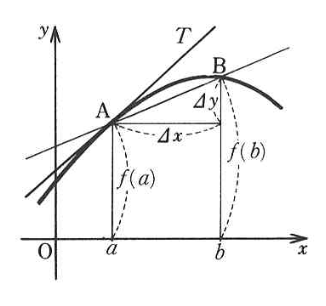
\includegraphics{source/images/intro/intro-1.png}

上の図のように, \(f(x)\) が \(x=a\) から \(x=b=a+\Delta x\)
だけ変化して場合に, \(\Delta y\)
だけの変化が起きるものとします.\(\Delta x,\; \Delta y\)
は一つの変数であり,増分と呼ばれます.

その時次の式が成り立つかと思われます.

\[\Delta y = \frac{f(b)-f(a)}{b-a} \Delta x\]

この式を次のように変形することによって,この式の概要が見やすくなるでしょう.

\[ f(b) = f(a) + \frac{\Delta y}{\Delta x}(b-a) \]

この式が表すものとは, \(f(b)\) の値が \(f(a)\) の値から
\(\frac{\Delta y}{\Delta x}(b-a)=\text{ABの傾き}\times a\text{と}b\text{の違いの分}\)
だけずれているということになるわけです.

この時, \(\frac{\Delta y}{\Delta x}\) の値を \(\Delta x\to 0\)
と極限をとって考えれば,ABの傾きは点Aにおける接線の傾きになるわけです.このとき,次のように書き記すことにします.

\[\lim_{\Delta x \to 0}\frac{\Delta y}{\Delta x}=\dv{y}{x}=y'=f'(x)\]

この値のことを微分係数と呼んでいます.先ほどの式を微分係数を使って書き直してあげれば次のようになるわけです.

\[ f(b) = f(a) + \frac{\Delta y}{\Delta x}(b-a) \]

\[ \Delta y = \dv{y}{x} \Delta x\]

ここで近似値にしたのは, \(\Delta x\)
をしっかりと極限とっていないからですが,今までやってきたことが接線を使って近似をしているというのがわかりやすい形なので採用しました.

この式の言わんとするところは,十分小さな \(\Delta x\) に関して言えば
\(\Delta y\) は接戦の傾きで近似できるということです.

以上のことを実際の具体的な関数でやってみましょう.例えば, \(f(x)=x^2\)
などを考えれば

\[\Delta y = \frac{b^2-a^2}{b-a} \Delta x = (b+a) \Delta x = (2a+\Delta x) \Delta x\]

と式変形がなされるわけです.これによって \(\Delta y,\; \Delta x\)
の比は次のように書き表され

\[\frac{\Delta y}{\Delta x} = 2a + \Delta x\]

となります.そして,極限を取ることによって

\[\dv{y}{x}=2a\]

となります.このことを \(f(x)\) の \(x=a\) における微分係数は \(2a\)
であると呼び,次のように表すことが多いです.

\[ \dv{y}{x}|_{x=a}=f'(a)=2a\]

また, \(a\) という具体的に代入した値ではなく,任意の \(x\)
についても同様なことが言えるため,

\[ \dv{y}{x}=f'(x)=2x\]

と書くことになります.この時, \(f(x)\) の導関数は \(f'(x)=2x\)
などと呼びます.以上の議論を最初から \(\Delta x,\: \Delta y\)
が微小分,つまり, \(\dd x,\: \dd y\) としてすることもでき,その場合は

\[\dd y = \frac{b^2-a^2}{b-a} \dd x = (b+a) \dd x = (2a+\dd x) \dd x = 2a \dd x + (\dd x)^2= 2a \dd x\]

\[\dv{y}{x} = 2a\]

ここで注目して欲しいのは, \(\dd y\) を表す式の中で, \(\dd x\)
の一次以上の項が消えていることです.これは極限を取ると消えてしまうからですね.

以上述べたように,微分を考える理由とは,接線で曲線を近似してみようという試みであり,また,曲線を非常に小さな部分で見てあげれば直線になると考えていることになります.

実際に問題を解いてみましょう.

\begin{Rbox}{例題}
次の関数の導関数を求めよ. \[f(x)=x^3+x+1\]

\end{Rbox}

\tcbox[arc is angular, shrink tight, extrude by=4pt]{解答}

\(a=x,\;b=a+\Delta x\) とする.
\[\Delta y = \frac{f(b)-f(a)}{b-a}\Delta x\]
\[\frac{f(b)-f(a)}{b-a}=\frac{f(a+\Delta x)-f(a)}{a+\Delta x -a} \]
\[= \frac{3x^2\Delta x + 3x\Delta x^2 + \Delta x ^3 + \Delta x}{\Delta x}\]
\[=3x^2+ 3x\Delta x + \Delta x ^2 + 1 \to_{\Delta x \to 0} 3x^2+1\]
\[\dv{y}{x}=3x^2+1\]

ここで注目して欲しいのは, \(\Delta y\) を表す式の中で, \(\Delta x\)
の2次以上の項が消えていることです.導関数を求める極限の計算では完全に消滅しますが,
\(\Delta x\) が \(0\)
に比較的に近いだけの値を考えている時の近似計算でも同様に無視したりします.このことを一次近似と呼んでいます.具体的な問題は後半にあるので,手を動かしてやってみましょう.

次に導関数に慣れてもらうために問題を置いておきます.

\begin{Qbox}{問題}

次の関数の導関数を求めよ.

\begin{longtable}[]{@{}ll@{}}
\toprule\noalign{}
\endhead
\bottomrule\noalign{}
\endlastfoot
\(x^2\) & \(\sqrt{x}\) \\
\((x+1)(x+2)\) & \(\frac{1}{x}\) \\
\(x\sqrt{x}\) & \(x^6+x^5+x^4\) \\
\end{longtable}

\end{Qbox}

\tcbox[arc is angular, shrink tight, extrude by=4pt]{解答}

\begin{longtable}[]{@{}
  >{\raggedright\arraybackslash}p{(\columnwidth - 2\tabcolsep) * \real{0.5000}}
  >{\raggedright\arraybackslash}p{(\columnwidth - 2\tabcolsep) * \real{0.5000}}@{}}
\toprule\noalign{}
\endhead
\bottomrule\noalign{}
\endlastfoot
\(2x\) &
\(\frac{\sqrt{x+\Delta x}-\sqrt{x}}{\sqrt{x}}=\frac{\Delta x}{\Delta x (\sqrt{x+\Delta x}+\sqrt{x})}\)
\(\frac{1}{2\sqrt{x}}\) \\
\(2x+3\) & \(-\frac{1}{x^2}\) \\
\(\frac{3}{2}\sqrt{x}\) & \(6x^5+5x^4+4x^3\) \\
\end{longtable}

\begin{Qbox}{問題}
次の極限値を \(f,f'\) を用いて表せ.

\[\lim_{x\to a}\frac{x^nf(x)-a^nf(a)}{x^n-a^n}\]

\end{Qbox}

\tcbox[arc is angular, shrink tight, extrude by=4pt]{解答}

\[f(a)+\frac{a}{n}f'(a)\]

\begin{Qbox}{問題}
次の値を近似して解け.

\[1024^2,\; \sqrt{74}\]

\end{Qbox}

\tcbox[arc is angular, shrink tight, extrude by=4pt]{解答}

\(f(x)=x^2\) とする. \[f(x+a) \approx f(x) + f'(x) \times a\] なので,
\(x=1000,\; a=24\) を代入することによって
\[1000^2 + 1000 \times 24 \approx 10024000\]

と近似できる.

後半の問題も同じく, \(f(x)=\sqrt{x},\; x=64,\; a=10\) とおいて解けば,
\[\sqrt{64+10} \approx \sqrt{64} + \frac{1}{2\sqrt{64}} \times 10 \approx 8.6 \]

\begin{Qbox}{問題}
次の事実を証明せよ.

\[(f+g)'=f'+g'\]

\[ (fg)' = f'g+fg'\]

\[\dv{x}\frac{1}{g}=-\frac{g'(x)}{\{g(x)\}^2}\]

\[\left\{ \frac{f}{g} \right\} ' = \frac{f'g-fg'}{g^2}\]

\[\dv{x} x^n = nx^{n-1}\]

\end{Qbox}

\tcbox[arc is angular, shrink tight, extrude by=4pt]{解答}

\((f+g)'=f'+g'\) は自力でせよ.

\$ (fg)' = f'g+fg'\$
は厳密な証明ではなく,一次近似を駆使して説明する.厳密な証明は自ら調べよ.

\[f(x+\Delta x)g(x+\Delta x) \approx (f(x)+f'(x)\Delta x)(g(x)+g'(x)\Delta x)\]

ここで二次以上の変化量( \(\Delta\) 付きの値)は無視されるので,
\[f(x+\Delta x)g(x+\Delta x) \approx f(x)g(x) + f'(x)g(x)\Delta x + f(x)g'(x)\Delta x\]
\[\frac{f(x+\Delta x)g(x+\Delta x)-f(x)g(x)}{\Delta x} = f'(x)g(x)+f(x)g'(x)\]

後半の問題は有名問題であり,今までの知識を使って自力で解決せよ.

最後の問題については二項定理を用いて自ら解決せよ.なおこの定理は \(n\)
が整数の時だけでなく,実数のときにも成り立つが,その証明は難しいのでここでは省略する.ただし,これからは使っていくので,知っておくこと.

ここで,このテキストの特徴として,詳しい解答を書いていないことが多々あることでしょう.これは,特定の問題までの内容を理解した人ならば違和感なく解ける問題や,有名すぎるあまりにわざわざ書くこともないだろうと思われる問題について当てはまることになります.ただし,ぜひともこの考え方を習得してもらいたいと思われる際には,詳しい解答を書くように心がけています.

また,この本では,読者が実際に手を動かして問題を解くことを前提にして書いており,問題と解答を読むだけではなかなか問題解決能力が身につかないのではないかと思われます.ご注意ください.

\hypertarget{ux5408ux6210ux95a2ux6570ux306eux5faeux5206ux6cd5}{%
\section{合成関数の微分法}\label{ux5408ux6210ux95a2ux6570ux306eux5faeux5206ux6cd5}}

次に次の問題を考えてみましょう.

\begin{Qbox}{問題}
次の事実を証明せよ.

\[y=x^2+x,\; z=y^3+1\] としたとき,次の値をそれぞれ求めよ.
\[\dv{y}{x},\;\dv{z}{y},\;\dv{z}{x}\]

\end{Qbox}

\[\dv{y}{x}=2x+1,\; \dv{z}{y}=3y^2\] これら二つは簡単でしょう.では,
\(\dv{z}{x}\)
はどうしたらいいでしょうか.分数と同様にするべきでしょうか.はい,その通りです.

\[\dv{z}{x}=3y^2(2x+1)=3(2x+1)(x^2+x)^2\]

\begin{Tbox}{定理}
\[\dv{y}{x}\cdot \dv{z}{y}=\dv{z}{x}\]

\end{Tbox}

証明は

\[\lim_{\Delta x \to 0}\frac{\Delta z}{\Delta x}=\lim_{\Delta x \to 0}\frac{\Delta z}{\Delta y}\frac{\Delta y}{\Delta x}\]

によって大まかに達成されます.ただし, \(\Delta y \neq 0\)
であることを前提にしている証明なので,厳密には証明になっていませんが,厳密な証明は難しいので省略させていただきます.

そして,この問題のおかげで私たちは次の問題を解決したことになるのです.

\(z=(x^2+x)^3+1\) の導関数を求めよ.

これを合成関数の微分法と呼ばれるもので,賢そうな人たちがチェーンルールと呼んでいるものです.

では,この定理を使って問題を解いていきましょう.

\begin{Rbox}{例題}
次の関数の導関数を求めよ. \[f(x)=\sqrt[3]{\frac{x^2}{1-x}}\]

\end{Rbox}

\tcbox[arc is angular, shrink tight, extrude by=4pt]{解答}

\(y=f(x),\; u=\frac{x^2}{1-x}\) とする.この時 \(y=\sqrt[3]{u}\)
となるため

\[\dv{y}{x}=\dv{y}{u}\dv{u}{x}=\frac{1}{3u^{2/3}}\frac{2x-x^2}{(1-x)^2}=\frac{1}{3}\left(\frac{1-x}{x^2}\right)^{2/3}\frac{2x-x^2}{(1-x)^2}\]

\begin{Qbox}{問題}
次の関数の導関数を求めよ.

\begin{longtable}[]{@{}
  >{\raggedright\arraybackslash}p{(\columnwidth - 2\tabcolsep) * \real{0.5000}}
  >{\raggedright\arraybackslash}p{(\columnwidth - 2\tabcolsep) * \real{0.5000}}@{}}
\toprule\noalign{}
\endhead
\bottomrule\noalign{}
\endlastfoot
\(\sqrt{a^2-x^2}\) & \(x+\sqrt{x^2-1}\) \\
\(\frac{x}{\sqrt{x^2+1}}\) &
\(\frac{\sqrt{a^2+x^2}-\sqrt{a^2-x^2}}{\sqrt{a^2+x^2}+\sqrt{a^2-x^2}}\) \\
\end{longtable}

\(x=y\sqrt{y+1}\) の時, \(\dv{y}{x}\) を求めよ.

\end{Qbox}

\tcbox[arc is angular, shrink tight, extrude by=4pt]{解答}

\begin{longtable}[]{@{}
  >{\raggedright\arraybackslash}p{(\columnwidth - 2\tabcolsep) * \real{0.5000}}
  >{\raggedright\arraybackslash}p{(\columnwidth - 2\tabcolsep) * \real{0.5000}}@{}}
\toprule\noalign{}
\endhead
\bottomrule\noalign{}
\endlastfoot
\(-\frac{x}{\sqrt{a^2-x^2}}\) & \(1+\frac{x}{\sqrt{x^2-1}}\) \\
\(\frac{1}{(x^2+1)\sqrt{x^2+1}}\) &
\(\frac{2a^2(a^2-\sqrt{a^4-x^4})}{x^3\sqrt{a^4-x^4}}\) \\
\end{longtable}

次の問題については,

\[\dv{x}{y}=\frac{3y+2}{2\sqrt{y+1}}\]
\[\dv{y}{x}=\frac{2\sqrt{y+1}}{3y+2}\]

これは逆関数の微分法と呼ばれるものだが,

\[\lim_{\Delta x \to 0}\frac{\Delta y}{\Delta x}=\lim_{\Delta x \to 0}\frac{1}{\frac{\Delta y}{\Delta x}}\]

を考えれば明らかである.ただしこの証明は連続性などの過程を飛ばした直感的なものに過ぎず,厳密な証明はここではしない.

\hypertarget{ux5897ux6e1b}{%
\section{増減}\label{ux5897ux6e1b}}

まず,定理から述べようと思います.

\begin{Tbox}{定理}

とある区間において,

\begin{itemize}
\tightlist
\item
  \(f'(x) \geq 0\) であれば,この区間では \(f(x)\) は増加する.
\item
  \(f'(x) \leq 0\) であれば,この区間では \(f(x)\) は減少する.
\end{itemize}

\end{Tbox}

この定理については,ある区間の内で接戦の傾きが常に正ならば,関数は増加し続ける,また逆も然りということを述べているわけです.この定理がどのように使われるかは,次の問題で話すことにしましょう.

\begin{Rbox}{例題}
次の関数のグラフの概形を描け. \[f(x)=x^3-3x+1\]

\end{Rbox}

\tcbox[arc is angular, shrink tight, extrude by=4pt]{解答}

\[f'(x)=3(x+1)(x-1)\]

導関数の形から,次のことが言える.

!\href{images/intro/intro-2.png}{}

この表のことは増減表と呼ばれる.初学のうちは書いておくと混乱が少ないが,慣れてきたのならばわざわざ書かなくとも良い.

上の増減表によってグラフの概形は次のようになる.

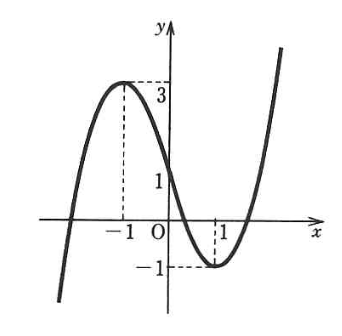
\includegraphics{source/images/intro/intro-3.png}

また, \(x=-1,\; x=1\)
の場所は増減が変化する点であり,この点のことを極大点,極小点などと呼んでいる.

\hypertarget{ux9762ux7a4dux3068ux533aux5206ux6c42ux7a4dux6cd5}{%
\section{面積と区分求積法}\label{ux9762ux7a4dux3068ux533aux5206ux6c42ux7a4dux6cd5}}

小学校以来,何となく扱ってきた「面積」というものについて,少し詳しく述べていきます.

まず,長方形の面積は「縦\(\times\)横」と決めましょう.このことについては特に異論はないと思います.この長方形の面積を手がかりに,いろいろな図形の面積,特にグラフと軸で囲われた部分の面積を考えていくことにしましょう.

\(xy\) 平面上で, \(y=f(x)\)
のグラフと,直線\(x=a,x=b\)で囲まれる領域の面積\(S\)を考えます.ここでは
\(f(x)\) は区間 \([a,b]\) で連続な関数であるとします.

(図)

このように,区間 \([a,b]\) を \(n\) 分割し,区間
\(\left[a+\displaystyle\frac{k-1}{n}(b-a),a+\displaystyle\frac{k}{n}(b-a)\right]\)
における \(f(x)\)の最大値を\(M_k\) ,最小値を \(m_k\)
とします.このとき,
\(\displaystyle\sum_{k=1}^{n}\displaystyle\frac{M_k}{n}\) は \(S\)
より少し大きく,
\(\displaystyle\sum_{k=1}^{n}\displaystyle\frac{m_k}{n}\) は \(S\)
より少し小さいことが下の図から分かると思います.

(図)

そして,この分割をどんどん細かくしたとき,すなわち\(n\to\infty\)のとき,\(\displaystyle\sum_{k=1}^{n}\displaystyle\frac{M_k}{n}\)および,\(\displaystyle\sum_{k=1}^{n}\displaystyle\frac{m_k}{n}\)
は \(S\) に限りなく近づくと考えられます.

上では各区間における \(f(x)\)
の最大値,最小値をとって考えましたが,実は区間
\(\left[a+\displaystyle\frac{k-1}{n}(b-a),a+\displaystyle\frac{k}{n}(b-a)\right]\)
ごとに好きな代表点 \(x_k\) をとって, \(M_k,m_k\) の代わりに \(f(x_k)\)
を考えても問題ありません.以上を踏まえて,
\[\displaystyle\lim_{n\to\infty} \displaystyle\sum_{k=1}^{n}\displaystyle\frac{b-a}{n}f(x_k)\]
を, \(y=f(x)\) のグラフと,直線\(x=a,x=b\)で囲まれる領域の面積 \(S\)
であると定めることにします.この考え方は,は区分求積法と呼ばれています.

\begin{Dbox}{定義}
\(y=f(x)\) のグラフと,直線\(x=a,x=b\)で囲まれる領域の面積 \(S\)を
\[\displaystyle\lim_{n\to\infty} \displaystyle\sum_{k=1}^{n}\displaystyle\frac{b-a}{n}f(x_k)\]
で定め,これを \[\displaystyle\int_{a}^{b}f(x)dx\] とかく.

\end{Dbox}

補足

ここで述べた面積(ついては積分)の定義は,正確なものではありませんが,少なくとも連続関数についてはこの定義で問題を生じないので,このまま進めることにします.

\begin{Qbox}{問題}
次の値を求めよ.ただし,代表点\(x_k\)は\(\displaystyle\frac{k}{n}\)とせよ.

\[\displaystyle\int_{0}^{1} x^2dx\]

\end{Qbox}

\tcbox[arc is angular, shrink tight, extrude by=4pt]{解答}

\begin{align*}
\displaystyle\int_{0}^{1} x^2dx &= \displaystyle\lim_{n\to\infty} \displaystyle\sum_{k=1}^{n}\displaystyle\frac{1}{n}\cdot \left(\displaystyle\frac{k}{n}\right)^2\\
&=\displaystyle\lim_{n\to\infty}\displaystyle\frac{1}{n^3}\displaystyle\sum_{k=1}^{n}k^2\\
&=\displaystyle\lim_{n\to\infty}\displaystyle\frac{1}{n^3}\cdot \displaystyle\frac{n(n+1)(2n+1)}{6}\\
&=\displaystyle\frac{1}{3}
\end{align*}

\hypertarget{ux5faeux5206ux7a4dux5206ux5b66ux306eux57faux672cux5b9aux7406}{%
\section{微分積分学の基本定理}\label{ux5faeux5206ux7a4dux5206ux5b66ux306eux57faux672cux5b9aux7406}}

1.7でみたように,面積の値を定積分として定めました.ここで,\(x\)を変数とした
\[\displaystyle\int_{a}^{x}f(t)dt\]
は,\(x\)の関数だと考えることができます.これを\(f(x)\)の不定積分と呼びます.

よく言われるように,微分と積分というのは互いに逆演算になっています.しかし,先の積分の項を読んだ方は,定積分の定義のどこにも微分が登場していない,ということにお気づきだと思います.実は微分と積分はそれぞれ独立して成立した分野で,後になって実は互いに関わりあっているということが分かったのです.

さて,次の定理は微分積分学の基本定理と呼ばれており,微分と積分を繋ぐ重要な事実です.

\begin{Tbox}{定理}
\[\displaystyle\frac{d}{dx}\displaystyle\int_{a}^{x}f(t)dt=f(x)\]

\end{Tbox}

これは,積分したものを微分すると元に戻る,ということを述べている定理です.この事実を使えば,わざわざ定義からいちいち積分をしなくても,「微分すると
\(f(x)\) になる関数」(これを原始関数といいます)を見つけられれば
\(f(x)\) の積分が求められる,ということになります.今後, \(f(x)\)
の不定積分は \(\displaystyle\int_{}^{}f(x)dx\) とかくことにします.

\begin{Rbox}{例題}
次の不定積分を求めよ. \[\displaystyle\int_{}^{}x\ dx \]

\end{Rbox}

\tcbox[arc is angular, shrink tight, extrude by=4pt]{解答}

微分の知識を思い出せば, \(\displaystyle\frac{1}{2}x^2\) の微分が \(x\)
になることはすぐにわかる.しかし,同様に
\(\displaystyle\frac{1}{2}x^2+1\) も,\(\displaystyle\frac{1}{2}x^2-99\)
も, \(\displaystyle\frac{1}{2}x^2+\pi\) も,
\(\displaystyle\frac{1}{2}x^2\)
に定数を足したものはすべて微分すれば\(x\)になる.これらをまとめて,
\(\displaystyle\frac{1}{2}x^2+C\)とかき,\(C\)を積分定数という.もとの例題に対する答えは,
\[\displaystyle\int_{}^{}x\ dx =\displaystyle\frac{1}{2}x^2+C~\mbox{($C$は積分定数)}\]
である.

上の例題のように,不定積分の結果には積分定数がつくことになります.都度但し書きを書くのは煩雑なので,積分の説明の間は「
\(C\) は積分定数」という説明は添えないことにします.

\begin{Qbox}{問題}

次の不定積分を求めよ.

\begin{longtable}[]{@{}
  >{\raggedright\arraybackslash}p{(\columnwidth - 2\tabcolsep) * \real{0.5000}}
  >{\raggedright\arraybackslash}p{(\columnwidth - 2\tabcolsep) * \real{0.5000}}@{}}
\toprule\noalign{}
\endhead
\bottomrule\noalign{}
\endlastfoot
\(\displaystyle\int_{}^{}1\ dx\) &
\(\displaystyle\int_{}^{}x^k\ dx\ \ \  ( k\neq -1 )\) \\
\(\displaystyle\int_{}^{}\displaystyle\frac{1}{x}\ dx\) &
\(\displaystyle\int_{}^{} \sin x\ dx\) \\
\(\displaystyle\int_{}^{}\cos x\ dx\) &
\(\displaystyle\int_{}^{} e^x\ dx\) \\
\end{longtable}

\end{Qbox}

\tcbox[arc is angular, shrink tight, extrude by=4pt]{解答}

前の説で述べた定積分の値については,不定積分を用いて計算することができます.

\begin{Tbox}{定理}
\(F(x)\) を \(f(x)\) の不定積分とすると
\[\displaystyle\int_{a}^{b}f(x)\ dx=F(b)-F(a)\] また,簡単のため
\(F(b)-F(a)\) のことを \(\left[F(x)\right]_{a}^{b}\) とかく.

\end{Tbox}

ここで,不定積分は積分定数がついていたことを思い出します.実は上の計算をするときは,積分定数の値について考慮する必要はなく,好きなもの(通常は0でしょう)を使って問題ありません.なぜなら,\(F(x)\)
の代わりに \(F(x)+C\) を使って右辺の計算をすると,引き算で結局 \(C\)
が消えてしまうからです.

\begin{Rbox}{例題}
次の定積分を求めよ. \[\displaystyle\int_{0}^{8}x\ dx \]

\end{Rbox}

\tcbox[arc is angular, shrink tight, extrude by=4pt]{解答}

\[\displaystyle\int_{}^{}x\ dx = \left[\displaystyle\frac{1}{2}x^2\right]_{0}^{8}=32-0=0\]

\begin{Qbox}{問題}

次の定積分を求めよ.

\begin{longtable}[]{@{}
  >{\raggedright\arraybackslash}p{(\columnwidth - 2\tabcolsep) * \real{0.5000}}
  >{\raggedright\arraybackslash}p{(\columnwidth - 2\tabcolsep) * \real{0.5000}}@{}}
\toprule\noalign{}
\endhead
\bottomrule\noalign{}
\endlastfoot
\(\displaystyle\int_{1}^{4}1\ dx\) &
\(\displaystyle\int_{0}^{1}x^k\ dx\ \ \  ( k\neq -1 )\) \\
\(\displaystyle\int_{1}^{e^2}\displaystyle\frac{1}{x}\ dx\) &
\(\displaystyle\int_{0}^{\pi} \sin x\ dx\) \\
\(\displaystyle\int_{-\frac{\pi}{3}}^{0}\cos x\ dx\) &
\(\displaystyle\int_{-1}^{1} e^x\ dx\) \\
\end{longtable}

\end{Qbox}

\tcbox[arc is angular, shrink tight, extrude by=4pt]{解答}

\hypertarget{ux7a4dux5206ux306eux7a2eux3005ux306eux6027ux8cea}{%
\section{積分の種々の性質}\label{ux7a4dux5206ux306eux7a2eux3005ux306eux6027ux8cea}}

この節では,不定積分や定積分の計算をする上で役に立つ色々な性質について説明し,それを使う練習をしていきます.

\begin{Tbox}{定理}
\(F(x)\) を \(f(x)\) の不定積分,\(G(x)\) を \(g(x)\)
の不定積分とし,\(a,b\) は定数とする.このとき,

\[\displaystyle\int_{}^{}(af(x)+bg(x))\ dx=aF(x)+bG(x)+C\]

これを積分の線形性という.

\[\displaystyle\int_{}^{}(af(x)+bg(x))\ dx=a\displaystyle\int_{}^{}f(x)\ dx+b\displaystyle\int_{}^{}g(x)\ dx\]

ともかける.

\end{Tbox}

\begin{tcolorbox}[enhanced jigsaw, colframe=quarto-callout-caution-color-frame, left=2mm, colbacktitle=quarto-callout-caution-color!10!white, rightrule=.15mm, bottomtitle=1mm, arc=.35mm, coltitle=black, title={例題}, titlerule=0mm, toptitle=1mm, toprule=.15mm, bottomrule=.15mm, leftrule=.75mm, opacitybacktitle=0.6, colback=white, opacityback=0, breakable]

次の定積分を求めよ. \[\displaystyle\int_{}^{}(2x+3x^2)\ dx \]

\end{tcolorbox}

\tcbox[arc is angular, shrink tight, extrude by=4pt]{解答}

\begin{align*}\displaystyle\int_{}^{}(2x+3x^2)\ dx &=2\displaystyle\int_{}^{}x\ dx+3\displaystyle\int_{}^{}x^2\ dx\\
&=x^2+x^3+C
\end{align*}

このとき,2つの不定積分の和では積分定数は \(C\)
だけでよく,2つつける必要はない.2つの不定積分から出てくる積分定数の和を改めて定数としておいてしまえばよいからである.

定積分についても,同様の公式が成り立つ.

\begin{Qbox}{問題}

次の不定積分や定積分を求めよ.現在ある問題は仮です.

\begin{longtable}[]{@{}
  >{\raggedright\arraybackslash}p{(\columnwidth - 2\tabcolsep) * \real{0.5000}}
  >{\raggedright\arraybackslash}p{(\columnwidth - 2\tabcolsep) * \real{0.5000}}@{}}
\toprule\noalign{}
\endhead
\bottomrule\noalign{}
\endlastfoot
\(\displaystyle\int_{1}^{4}1\ dx\) &
\(\displaystyle\int_{0}^{1}x^k\ dx\ \ \  ( k\neq -1 )\) \\
\(\displaystyle\int_{1}^{e^2}\displaystyle\frac{1}{x}\ dx\) &
\(\displaystyle\int_{0}^{\pi} \sin x\ dx\) \\
\(\displaystyle\int_{-\frac{\pi}{3}}^{0}\cos x\ dx\) &
\(\displaystyle\int_{-1}^{1} e^x\ dx\) \\
\end{longtable}

\end{Qbox}

\tcbox[arc is angular, shrink tight, extrude by=4pt]{解答}

\bookmarksetup{startatroot}

\hypertarget{ux4f4dux7f6eux901fux5ea6ux52a0ux901fux5ea6}{%
\chapter{位置,速度,加速度}\label{ux4f4dux7f6eux901fux5ea6ux52a0ux901fux5ea6}}

この章では主に速度とか加速度についてお話しさせていただきます.

\hypertarget{ux7269ux7406ux306bux3064ux3044ux3066}{%
\section{物理について}\label{ux7269ux7406ux306bux3064ux3044ux3066}}

まず,物理の話を始める際において,物理は何かということを明らかにしなければなりません.ところが物理とは何かという問題はあまりに大雑把で,人によってその定義が変わるものだし,専門とする分野によっても大きく姿を変えることでしょう.ですが,それらを全てまとめ上げ,最大公約数的な解答を一つ提示できるとすれば,私たちの身の回りで起きている,現象について語る学問だということになるのではないかと思います.

例えば,皆さんがこの本をパソコン越しでみているとします.その時,パソコンに映る表示映像というのも何らかの現象でしょう.ではその現象を観察し,何か語れるものがあるのかと考えてみましょう.例えば,「あ」という文字と「あ」という文字は全くもって同じ形をしているという法則が見つけられるかもしれません.マウスホイールを回すとテキストが流れていくという法則も見えてくるでしょう.

ところが現象とざっくり言ってしまっては,どの現象をどの角度から見ることになるかがはっきりしてきません.では,私たちがこれから学ぶ物理学の,ひとまず注視することとなる現象を考えることから始めましょう.その現象とは,動く物体です.

ここでは話がわかりやすくイメージできるように,とあるパチンコ玉を考えてみましょう.そのパチンコ玉は机の上に置かれていて,手で弾いてやると机の上をまっすぐ転がっていき,やがて机の淵から落ちて地面と衝突し,数度バウンスしたのちに床で止まりました.

さて,この現象を語るのに今は日本語という言葉を使いましたが,これでパチンコ玉の運動の仔細は語り尽くされたのでしょうか.弾き飛ばされたパチンコ玉がどれくらい早く動き,机に対してどんな角度で転がって,机の淵までどれくらいの時間で辿り着き,バウンスによってどれだけの高さに跳ね上がり,どの場所でその動きを止めたのか.少なくともこれらの情報がなければ,現象を語られた人が同一の現象を想定することは不可能でしょう.また,これらの情報を渡されたところで,全く同じ現象を想定するのも難しいに違いありません.そしてその再現度こそが,現象を語り尽くすことの根幹なのではないでしょうか.

では,どうすれば,パチンコ玉の運動を語り尽くせるのでしょうか.その時に使われるのが,数学の力なのです.

\hypertarget{ux901fux5ea6ux53caux3073ux52a0ux901fux5ea6}{%
\section{速度及び加速度}\label{ux901fux5ea6ux53caux3073ux52a0ux901fux5ea6}}

パチンコ玉の中心点の座標 \(\boldsymbol{r}\) を,時間 \(t\)
ごとに追っていって,その全ての時間に対して解析を行い,時間の関数となる
\(\boldsymbol{r}(t)\)
を書き上げれば,上に書かれたすべての疑問に対して回答することができ,さらには現象を語り尽くすことができるのではないでしょうか.もっと具体的に言えば,パチンコ玉の回転なども考慮すべきでしょうが,今の所,それは無視することにします.

では,今,私たちはパチンコ玉の運動を語り尽くす手段を知りました.では,その運動の様相をどのようにして解析するのかを考える段階に入りましょう.確かに,パチンコ玉は
\(\boldsymbol{r}(t)\)
に従って動いていますが,我々の直感として「動いている」と感じることのできる指標である「速さ」が必要になるでしょう.動いているか,動いていないかの判別にも使えるし,動いている様相の説明にも使えるでしょう.

また,物理学という学問の性質上,古の巨人が築き上げた知識を引き継ぐことが大いにありますが,ニュートンの語るところによれば,物体の運動において大きな役割を持つ指標が加速度であるので,それも合わせて定義していくことにします.

\begin{Dbox}{定義}
とある物体の時刻 \(t\) における位置ベクトルを \(\boldsymbol{r}(t)\)
とした時、

その物体の速度を
\[\boldsymbol{v}(t)=\frac{d\boldsymbol{r}}{dt}=\dot{\boldsymbol{r}}\]

加速度を
\[\boldsymbol{a}(t)=\frac{d^2\boldsymbol{r}}{dt^2}=\ddot{\boldsymbol{r}}=\dot{\boldsymbol{v}}\]

と定義する。また、 \[\boldsymbol{r}(0),\boldsymbol{v}(0)\]
をそれぞれ初期位置、初速度と呼び,速度の絶対値を速さと呼ぶ.

\end{Dbox}

速度とは,わずかな時間における時間あたりの位置の変化です.つまり,そのわずかな時間をかけてやることによって,わずかな時間に起きた位置の変化を求めることができ,さらに,そのわずかな時間に起きた位置の変化を全て足し合わせることによって,位置を求めることができるのです.

ここで, \(t=0\) から \(t=T\) までの時間を \(n\)
個に区切り,その一区切りの時間の長さを \(\Delta t\) , \(i\)
区切り目の時刻を \(t_i\) としてやれば,

\[\boldsymbol{r}(t)\approx\sum_{i=0}^n \boldsymbol{v}(t_i)\Delta t\]

とすることができ,極限をとってあげることによって

\[\boldsymbol{r}(t)= \lim_{\Delta t \to 0}\sum_{i=0}^n \boldsymbol{v}(t_i)\Delta t=\int \boldsymbol{v}(t_i)\dd t\]

となるわけです.同様の話が加速度についても言えます.では,これからは実際に例題を用いて,今までの知識を深めていきましょう.

\begin{Rbox}{例題}
\(x\) 方向への一次元で,速度が一定 \(v\)
の物体の運動を考える.最初物体は \(x=x_0\) にあったとして,時刻が
\(t=T\) になった時の位置を求めよ.

\end{Rbox}

\tcbox[arc is angular, shrink tight, extrude by=4pt]{解答}

まず, \(x=x_0\) から \(t=T\)
だけ経った時に物体がどれだけ動いたか考えると

\[\int_0^T v \dd t=vT\]

なので, \(x_0+vT\) が答えになる.

次に別の方法を考えると,

\[x=\int v \dd t = vt+C\]

であるので,初期条件の \(t=0,\; x=x_0\) を代入すると

\[x = vt + x_0\]

ここで,積分が定積分ではなく,不定積分であることに注目せよ.定積分でない理由は,この場合,
\(x\)
を求めるのに,微分の逆演算をしているに過ぎず,ある定まった区間での積分として考えていない.

次の問題では,一次元の等加速度運動を全てまとめているものになります.

\begin{Rbox}{例題}
\(x\) 方向への一次元で,加速度が一定 \(a\) の物体の運動を考える.時刻
\(t=t_0\) 物体は \(x=x_0,\; v=v_0\) だったとして,時刻が \(t\)
になった時の位置を求めよ.

\end{Rbox}

\tcbox[arc is angular, shrink tight, extrude by=4pt]{解答}

前の問題の結果を使えば,

\[v=v_0+\int_{t_0}^{t}v\dd t = v_0 + a(t-t_0)\]

この解答は \((t-t_o)\) を一塊としてみて,先の問題の \(T\)
のように扱っている.塊として考えればこれからの問題も比較的楽に解決される.ここでは
\(T=t-t_0\) とすれば,

\[v=v_0 + aT\]

\[x-x_0=\int_{0}^{T}v\dd t =\frac{1}{2}aT^2+v_0T\]

\[x = \frac{1}{2}aT^2+v_0T + x_0\]

このように扱うことができるわけだが,読者が問題解決の際には \(T\)
をわざわざ定義しなくとも,塊のまま見てあげることによって,

\[x = \frac{1}{2}a(t-t_0)^2+v_0(t-t_0) + x_0\]

としてあげれば良い.

\hypertarget{ux91cdux529bux52a0ux901fux5ea6}{%
\section{重力加速度}\label{ux91cdux529bux52a0ux901fux5ea6}}

では,先述した,加速度が物理において重要な役割を持つ理由について少し話しましょう.

地上において,支えをなくした物体が自由落下するという現象について,人類は長い間色々な議論を作り上げました.その中でもおそらく最も正確に現象に忠実な解釈は「自由落下する物体は常に鉛直方法下向きに一定の加速度を持つ」というものでしょう.その加速度の大きさは重力加速度といわれ,
\(g=9.8\:\text{m}/\text{s}^2\)
と測定されています.この本ではこれから特に断りなく \(g\)
を重力加速度として扱っていくのでご注意ください.

簡単な例として,鉛直上向きに \(y\) 軸を設定し,初期位置が \(y=y_0\)
である物体の自由落下を記述してみましょう.

\[\ddot{y}=-g\] \[\dot{y}=-gt\] \[y=y_0-\frac{1}{2}gt^2\]

\hypertarget{ux76f8ux5bfeux4f4dux7f6eux76f8ux5bfeux901fux5ea6ux76f8ux5bfeux52a0ux901fux5ea6}{%
\section{相対位置,相対速度,相対加速度}\label{ux76f8ux5bfeux4f4dux7f6eux76f8ux5bfeux901fux5ea6ux76f8ux5bfeux52a0ux901fux5ea6}}

次に,相対位置の定義だけ少し説明します.ベクトルになれた読者の方にとって,あまり難しい概念ではないので,定義だけ載せます.

\begin{Dbox}{定義}
とある2つの物体の位置ベクトルを \(\boldsymbol{r_1},\;\boldsymbol{r_2}\)
とした時、

物体2の,物体1から見た相対位置ベクトルを

\[\boldsymbol{r_{21}}=\boldsymbol{r_2}-\boldsymbol{r_1}\]

と定義し,相対速度,相対加速度も同様にして定義する.

\end{Dbox}

ここで,相対速度があれば,絶対速度というものも存在するのではないかという疑問が湧くことかと思います.

//TODO 絶対速度のないことと,系についての説明

では,実際の問題を解きながら,加速度と速度について慣れていきましょう.

\begin{Rbox}{例題}

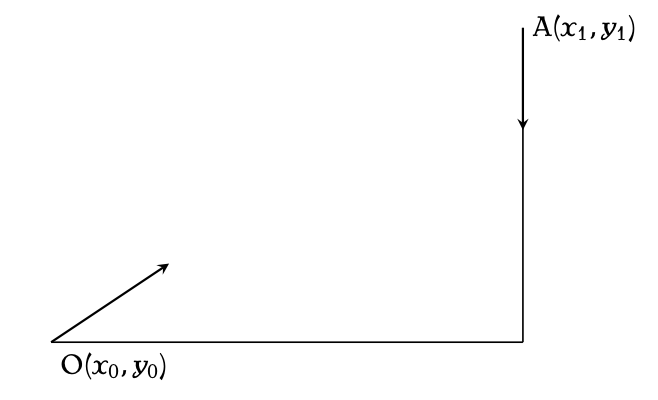
\includegraphics{source/images/velocity/mondai2.png}

図の通り \(O,A\) に物体 \(o,a\)
があり、それらをそれぞれ違う速度で同時に射出する機構がある。全ての物体が鉛直下向きに大きさ
\(g\) の加速度を受ける状態にある。物体 \(o\) を初速度の大きさ \(v_0\)
で射出し、射出される角度を水平方向から見て上方向に \(\theta\)
とする時、次の問いに答えよ。

\begin{enumerate}
\def\labelenumi{\arabic{enumi}.}
\item
  物体 \(o\) の軌跡を求めよ.
\item
  物体 \(o\)
  がはじめと同じ高さの地点を通過する際、最も水平方向遠方へと射出される
  \(\theta\) の条件を求めよ。
\item
  物体 \(a\) が初速度0で射出された場合、物体 \(a\) の物体 \(0\)
  から見た相対位置ベクトルはどうなるか。
\item
  物体 \(a\) が初速度0で射出された場合、2物体が衝突する \(\theta\)
  の条件を求めよ。
\item
  物体 \(a\) が鉛直下向きに大きさ \(v_1\)
  初速度で射出された場合、2物体が衝突する \(\theta\) の条件を求めよ。
\item
  全ての物体が鉛直下向きに大きさ \(g\)
  の加速度を受ける状態にあるとして今までの問題を解いてきたが、その条件を取り払い、代わりに、全ての物体が水平右向きに大きさ\(h\)の加速度を受ける状態にあるとすると、問題2,3の結果はどうなるか。
\end{enumerate}

\end{Rbox}

\tcbox[arc is angular, shrink tight, extrude by=4pt]{解答}

\begin{enumerate}
\def\labelenumi{\arabic{enumi}.}
\item
  時刻\(t\)における物体 \(o\) の加速度は \((0,-g)\)
  となるので、これを積分すれば速度がもとまる.ベクトルの積分は各要素それぞれに対して行えばいいだけなので、
  \(\boldsymbol{v}(t)=(C_1,C_2-gt)\) となる。ここで積分定数である
  \(C_1,C_2\) を決めていくこととなる.\[ \]
  数学では不定積分は積分定数を放置したままやっていたことが多いと思われるが、物理では積分定数を決めなければならないことが多い。その理由は、数学では微分をすることによって元の関数に戻る関数群を求めていたと言う作業をしていたが、物理ではそのような関数群のうち、現実を記述していると思われる一つの関数を定めるからである。同時に二つ以上の速度を持つ物体というものは存在しないのだ。\[ \]
  では、どのようにして積分定数を求めていくかというと、前の0台と同じく,与えられた条件を代入すれば良い。同時に二つ以上の速度を持たない物体なのであれば、任意の時刻において一つの速度を持つはずである。この問題の場合、射出時に
  \((v_0\cos \theta, v_0 \sin \theta)\)
  の速度を持つことが与えられた条件で,このときの時刻を \(t_0\)
  とでもおいてやれば、
  \(\boldsymbol{v}(t_0)=(v_0\cos \theta, v_0 \sin \theta)\)
  という方程式になる。これによって
  \(\boldsymbol{v}(t_0)=(v_0\cos \theta, v_0 \sin \theta-g(t-t_0))\)
  ともとまる。\[ \] 賢明な読者の方は開始時刻を \(t_0\)
  と置くのはエレファントな考え方であるというかもしれない。その通りである。開始時刻を
  \(0\)
  にすればもっと単純な式になる。だが,せっかくの例題なので,あえて面倒な方で解いても解けることをまず示しておこうと思う.\[ \]
  さて、解答の続きに戻ると、\(\boldsymbol{v}\) によって物体 \(o\) の座標
  \(\boldsymbol{r}\) を求めないことには話は始まらない。ならば、
  \(\boldsymbol{v}\) を再び \(t\) で積分してやって、時刻 \(t_0\)
  における物体 \(o\) の座標 \((x_0,y_0)\)
  でもって積分定数を求めてやれと、そう考えるのが先の発想であった。ここでは
  \(t-t_0\) という塊で考える。そうすれば自然と次が求める物体 \(o\)
  の座標になるわけである.
  \[\boldsymbol{r}(t)=(x_0+v_0\cos \theta (t-t_0), y_0+v_0 \sin \theta (t-t_0)-\frac{1}{2}g(t-t_0)^2)\]
  同様に, \(t-t_0\) を塊としてみて,計算を続ければ軌跡は
  \[y=y_0+(x-x_0)\tan\theta-\frac{g}{2}\frac{(x-x_0)^2}{v_0^2\cos^2\theta}\]
  と,求まる.
\item
  結論を言えば、 \(r_y=y_0\) となる \(t\)
  は \(t-t_0=0,\frac{2v_o\sin\theta}{g}\) で、後者を \(r_x\) に代入し、
  \[r_x=x_0+\frac{2v_0^2}{g}\sin \theta \cos \theta=x_0+\frac{v_0^2}{g}\sin 2\theta\]
  となることから、求める条件は\(\theta = \pi /4\)となる.とても直感にあった結果となったと思う.
\item
  この問題の作業は問題1と同じなので、略解のみを書く。求めるベクトルは
  \(T=t-t_0\) として,
  \[\boldsymbol{r}_r=(x_1-x_0-v_0\cos\theta T,y_1-y_0-v_0\sin\theta T)\]
\item
  \(\boldsymbol{r}_r=\boldsymbol{0}\) となる \(T\)
  が存在することが条件なので、
  \[\theta = \tan ^{-1} \frac{y_1-y_0}{x_1-x_0}\] すなわち、最初から物体
  \(o\) を物体 \(a\)
  に向けて発射さえすれば良いというのが、結論である。この次の問題である問題2をやれば、この問題を相対運動で見てやればただの等速運動問題であるとわかっていただけるだろう.
\item
  この場合の相対速度が
  \[\boldsymbol{r}_r=(x_1-x_0-v_0\cos\theta T,y_1-y_0-(v_0\sin\theta +v_1) T)\]
  であることは、容易にわかるではないかと思う。なので求める条件は
  \[\frac{\sin\theta + v_1/v_0}{\cos\theta} = \frac{y_1-y_0}{x_1-x_0}\]
  となります。
\item
  実際に各物体の座標を計算してみるのもいいが、両物体の座標が共通して持つ項は、相対位置ベクトルを計算する際に相殺されてしまう.例えばこの問題で言えば、両物体がどの方向であろうとも、同じような加速度を受ける状態なんであれば、
  \[\boldsymbol{r}_r=(x_1-x_0-v_0\cos\theta T,y_1-y_0-v_0\sin\theta T)\]
  は変わらないです。ゆえに結果は変わりはない。加速度のみならず、速度や変位に関しても同じことが言えることにも注意せよ。
\end{enumerate}

最後に放物運動についての重要な性質をいくつか書いておく.

\begin{itemize}
\tightlist
\item
  放物開始点から最高点に達するまでの時間と,最高点から下の高さまで戻る時間は等しい
\item
  同じ高さでは同じ速さとなる
\end{itemize}

\begin{Qbox}{問題}

ある車が静止から加速度 \(a\) で動き出した.同時に,同じ開始地点に速さ
\(v\) のトラックが通過した.この時次の問を答えよ.

\begin{enumerate}
\def\labelenumi{\arabic{enumi}.}
\item
  車とトラックが再びすれ違うまで,どれだけの時間がかかったか
\item
  車とトラックが再びすれ違うまで,車はどれほど進んだか
\item
  車とトラックが再びすれ違う際の車の速度はいかほどか
\end{enumerate}

\end{Qbox}

\tcbox[arc is angular, shrink tight, extrude by=4pt]{解答}

車とトラックの原点から見た位置をそれぞれ \(x_1,\: x_2\)
とした時,次の式が成り立つ.

\[x_1=\frac{1}{2}at^2,\;x_2=vt\]

車とトラックがすれ違う時間は \(x_1=x_2\) で求まるので,
\[\underline{t=\frac{2v}{a}}\] 次に進んだ距離 \(s\) は
\[s=\frac{2v^2}{a}\] 車の速さ \(V\) は \[V=2v\] となる.

\begin{Qbox}{問題}

\begin{enumerate}
\def\labelenumi{\arabic{enumi}.}
\tightlist
\item
  次の等式を示せ.
\end{enumerate}

\[\int \ddot{x} dx = \frac{1}{2}v^2 + C\] 特に \(\ddot{x}=a\)
と加速度が一定の際,初速度 \(v_0\) から運動を始めて \(x\)
だけ進んだ物体の速さを \(V\) として, \[v^2-v_0^2=2ax\]
が成り立つことを示せ.

\end{Qbox}

\tcbox[arc is angular, shrink tight, extrude by=4pt]{解答}

\[\int a\dd x=\int \dot{v}\dv{x}{t}\dd t = \int \dot{v}v\dd t=\frac{1}{2}v^2 +C\]
問題後半については,
\[\int_{0}^{x}a\dd x=\int_{0}^{T}\dot{v}\dv{x}{t}\dd t = \int_{0}^{T}\dot{v}v\dd t=\left[\frac{1}{2}v^2\right]_{0}^{T}=\frac{1}{2}(V^2-v_0^2)\]
\[\int_{0}^{x}a\dd x=ax\] から導き出される.

\begin{Qbox}{問題}
(アデレード大)

鉛直上向き正の \(y\)
軸の原点から\textbf{下に離れた位置}から,鉛直上向きにある物体を投げ上げた時,その物体の高さ
\(y=-h\) の時の速さが,高さ \(y=h\)
の時の速さの2倍になったという.この時,この物体の最高到達位置を求めよ.

\end{Qbox}

\tcbox[arc is angular, shrink tight, extrude by=4pt]{解答}

高さ \(y=0,\:h\) の時の速さをそれぞれ \(u,v\) とした時,次の式が成り立つ
\[v^2-u^2=-2gh\] \[(2v)^2-u^2=2gh\] この式から \(v\)
を消すことによって次の式が成り立つ \[u^2=\frac{10}{3}gh\]
最後にこの物体がたどり着ける最高点の高さを \(H\) とした時,
\[H=\frac{u^2}{2g}=\frac{5}{3}h\] となることがわかる.

\begin{Qbox}{問題}
ある粒子が下の図のような加速度で移動したとする.初速を \(v_0\)
とした時, \(x=3x_0\)
の時の速さを求めよ.\textbf{ただし,横軸が時間ではなく座標であることに注意せよ.}

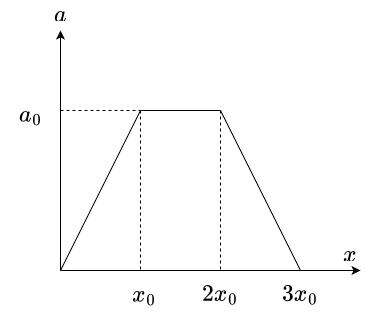
\includegraphics{source/images/velocity/mondai1-re.png}

\end{Qbox}

\tcbox[arc is angular, shrink tight, extrude by=4pt]{解答}

\[\int_{0}^{3x_0}a\dd x=\int_{0}^{T}\dot{v}\dv{x}{t}\dd t = \int_{0}^{T}\dot{v}v\dd t=\left[\frac{1}{2}v^2\right]_{0}^{T}=\frac{1}{2}(V^2-v_0^2)\]

また,台形の面積により,

\[\int_{0}^{3x_0}a\dd x = 2a_0x_0\]

\[V=\sqrt{v_0^2+4a_0x_0}\]

\begin{Qbox}{問題}
幅が\(L\)で、ある地点から河岸までの両距離を \(\delta_1,\delta_2\)
とした時、その地点での流速が \(k\delta_1\delta_2\)
となる川があり、それを速さ \(v\)
の船で横断することを考える。船首は常に対岸に真っ直ぐ向いているとして、この船が描く軌跡はどうなるか。適当に座標を設定して答えよ。

\end{Qbox}

\tcbox[arc is angular, shrink tight, extrude by=4pt]{解答}

川の流れる方向を \(y\) 軸,船の進む方向を \(x\)
軸,船の最初いる場所を原点として、 \(xy\) 座標を考える。船のいる座標は
\(\boldsymbol{r}=(x,y)\) である時、川の流れは \(kx(L-x)\) となるので、
\(\boldsymbol{v}=(v,kx(L-x))\) となる。ここで、 \(x=vt\) から、
\(v_y=kvt(L-vt)\) となり、実際に積分計算をしてやると、
\(y=kvL\frac{t^2}{2}-kv^2\frac{t^3}{3}\)
となり、軌跡を出さないといけないので \(t\) を代入をしてやれば、
\[y=\frac{kL}{2v}x^2-\frac{k}{3v}x^3\] が答えになる。

\begin{Qbox}{問題}
2輌の燃料タンクが積まれた車A,Bがあり、それぞれ2種類のエンジンを搭載している。これらのエンジンの効率などを計測するために、2輌の車を同じ長さのテストコースで走らせる。Aは丁度コースの半分まで加速し続け、その後は等速でコースを走り去った。Bはコースの最後まで加速し続けた。奇しくもA,Bは同時刻に発射し、同時刻にゴールに達した。A,Bの加速度の比と、ゴール時の速度の比を求めよ。

\end{Qbox}

\tcbox[arc is angular, shrink tight, extrude by=4pt]{解答}

コースの長さを \(L\) 、それぞれの車の加速度を \(a_A,a_B\)
、最大速度に達する時間を \(t,T\) とおくと次のような方程式が成り立つ.
\[L=\frac{1}{2}a_At^2+a_At(T-t)\] \[L=\frac{1}{2}a_BT^2\]
\[\frac{1}{2}L=\frac{1}{2}a_At^2\]
これらの方程式は未知数が5つあるので、一見解決は無理そうに見えますが、全ての式が
\(L\)
だけの変数を持つ左辺を持つ事実と、右辺の字数が全て揃っているところから解決が可能である。実際、1,2番目の式を3番目の式で割ってやれば、
\(a_A/a_B,T/t\)
の二つを未知数と見立てた方程式が出来上がり、実際に計算してやると、
\[\frac{a_A}{a_B}=\frac{9}{8},\;\frac{a_At}{a_BT}=\frac{3}{4}\]
が求める比になる。

\begin{Qbox}{問題}
一定の流速の川でモーターボートとイカダが動いている.モーターボートは川の流速に対して一定の速度を保ちながら動いており,また,イカダは動力を持たずに川に流されているものとする.

モーターボートはある地点Aでイカダを通り越し,それから時間 \(t\)
後に地点Bで引き返し,再び地点Cでイカダとすれ違った.地点Aと地点Bの距離は
\(l\) であるとして,この川の流速を求めよ.

\end{Qbox}

\tcbox[arc is angular, shrink tight, extrude by=4pt]{解答}

流速とともに動く座標系で考える(もしこの考え方に馴染みがなければ,最初は飛ばしても良い).この時,イカダは常に止まっており,モーターボードのみがイカダから離れては戻ってくる運動をする.この時,行きと戻りは,同じ距離を同じ速さで動いているので,ともに同じ時間
\(t\) だけかかり,合計 \(2t\)
だけかかったことになる.ここで川に対してとまっている,地面に対して静止している座標系で考えた時,イカダは
\(l\) だけ動いたことになる.つまり,イカダは \(2t\) の時間で \(l\)
だけ動いたことになり,流速は \(l/2t\) と求まる.

次に少しだけだが煩雑な考え方をする. \(AB=BC+l\)
なので,モーターボートが引き返したのちにイカダとすれ違うまでの時間を
\(t'\) ,ボートのかわに対する速さを \(V\) とすると \[(V+v)t=l+(V-v)t'\]
また,イカダは時間 \(t'\) の間に \(l\) だけ進んでいるので, \[vt'=l\]
これらを連立することによって \[v=\frac{l}{2t}\] とわかる.

\hypertarget{ux96e3ux554fux30d1ux30fcux30c8}{%
\subsection{難問パート}\label{ux96e3ux554fux30d1ux30fcux30c8}}

これからの問題に対する直感的な解決法は問題の解答の後半にあるので、前半の記述が難しいと感じられたのであれば、スキップしてお読みいただければ嬉しいです。

\begin{Qbox}{問題}
\(x=0\) で固定された長さが最初 \(x=L\)
まである鉄板の端に車輪が立っており、鉄板は \(x\)
軸プラス方向に無限に、均等に伸び続ける。また、車輪は鉄板に対して一定の速さ
\(v\) で \(x\) 軸マイナス方向に進み続ける。この時、車輪が \(x=0\)
にまで辿り着く条件はどうなるか?

\end{Qbox}

\tcbox[arc is angular, shrink tight, extrude by=4pt]{解答}

鉄板と車輪の速さを \(v,c\)
とする。まず鉄板上を無数の点があると考える。鉄板が伸びるというのは、これらの無数の点の間隔が伸びることを意味する。次に、時刻
\(t\) の時を考える。伸びる前における座標 \(x\) の点上から座標
\(x-\dd x\) の点まで、車輪がマイナス方向に転がる時間が \(\dd t\)
であるとする。二つの点の距離は鉄板の伸びから \(\frac{L+vt}{L}\dd x\)
で、これを \(\dd t\) の時間で進むので、 \(c\dd t\)
となり、次の式が成り立つ。 \[\frac{L+vt}{L}\dd x=c\dd t\]
\[\dd x=\frac{c}{1+vt/L}\dd t\] 両辺を \(0\) から \(T\) 積分してやれば
\[x=\frac{Lc}{v}\ln \frac{L+vT}{L}\] ここで求めた \(x\) とは、時間 \(T\)
までに車輪が進んだ距離の、伸びる前における座標の換算になります。つまり、
\(x=L\) を代入して、求めた \(T\) の \[T=\frac{L}{v}(e^{\frac{v}{c}}-1)\]
が端にまで辿り着く時間となる。つまり、問題の答えとしては、伸びる速さがどれほどはやくとも、車輪がどれほどノロノロしていようと、鉄板が最初どれほど長かろうとも、有限の時間で絶対に車輪は端にたどり着くということである。\textbackslash{}
一見不思議な結果のように思われるかもしないが、実は少しだけ考え方を変えてやれば簡単に解決する。\textbackslash{}

\textbf{後半部分}

車輪は常に \(x\)
軸マイナス方向に進み続けているのだが、鉄板が伸びる速さがどれほどのものとなろうとも、伸びる前換算でプラス方向に進むことはあり得ない。なぜなら、車輪は常に鉄板に対して、その伸びる方向と逆方向に速さを持っているからである。なので、いつか絶対に端にたどり着くのだ。

\begin{Qbox}{問題}
一辺100メートルの正方形の各頂点に人A ,B
,C,Dが立っている。時刻0に秒速1メートルでAはBに向かい、BはC、CはD、DはAに向かって歩き始める。歩いている間は各々は自分が向かっていた相手を目指し続けて歩くとする。人を質点として考えるとき、彼らは出会うことはあるか。もしも出会うなら、彼らは何秒で出会い、どれだけの距離を歩き、最終地点の周りを何回周ったことになるか。また,正方形ではなく,正三角形だった場合はどうなるか.

\end{Qbox}

\tcbox[arc is angular, shrink tight, extrude by=4pt]{解答}

具体的にそれぞれの人の歩く軌跡をデカルト座標で考えていくとすれば非常な困難に立ちはだかることが予想される。では、人の動き方が、対称性から四人が常に四角形を成す位置にあり、ぐるぐる周っていくことから、極座標での解決の仕方はどうだろうか。
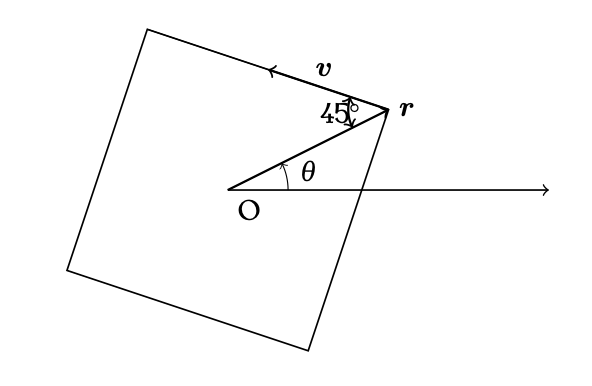
\includegraphics{source/images/velocity/mondai3.png}
以上の図によって、おおよそ人のいつ場所と速度を考えることができる。ここで、時間を追って
\(r,\theta\) がどのように動くかを考えてみると、次の図のようになる。
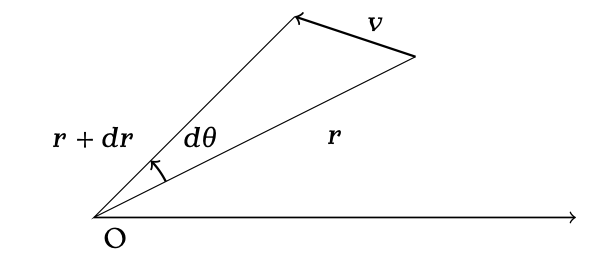
\includegraphics{source/images/velocity/mondai4.png} \(r,v\)
の作る角度などから、次の2つの式を求めることができる.
\[dr=-v\cos 45^\circ dt\] \[\tan 45 ^\circ = \frac{rd\theta}{dr}\]
\(t=0\)の時、\(r=R,\theta=0\)として、微分方程式を解いていくことによって、
\[r=R-\frac{v}{\sqrt{2}}t\] \[d\theta=\frac{dr}{r}\] \[r=Re^{-\theta}\]
\[\theta = \ln \frac{R}{R-\frac{v}{\sqrt{2}}t}\] のように \(r,\theta\)
を \(t\) の関数で表すことができる。これらの式からA ,B
,C,Dが出会う時刻は \(\sqrt{2}R/v\) となり、無限回最終地点の周りを周ったことになる。では、彼らがどれだけ歩いたことになるのだろうか。この問題は次のように解決される。
\[\int_0^\infty \sqrt{r^2+(\frac{dr}{d\theta})^2} d\theta=\sqrt{2}R\]
正三角形の場合も似たような議論が可能であるが,省略する.

\textbf{後半部分}

Bから見たAの相対速さは,AとBの速度が常に垂直なので, \(1\)
メートル毎秒となり、 \(100\) 秒後に \(100\)
メートルに歩いて出会うことになる。対称性から無限回回転するか、一回も回転しないかどちらかで、明らかに後者ではないということもわかる。

正三角形の場合は別の考え方をする.

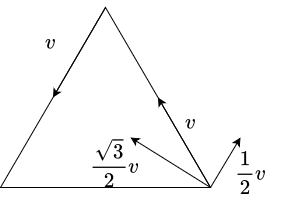
\includegraphics{source/images/velocity/mondai5.png}

図のようにAは常に三角形の中心に向かって \(\sqrt{3}v/2\)
の速さで進むことになる.三角形の中心からAまでの最初の距離は
\(100/\sqrt{3}\) メートルなので,かかる時間は \(200/3\)
秒である.また,お互いに向かって歩いている割合は図からわかるように
\(1:2\) なので,進む距離は \(100\times 2/3=200/3\) mである.

\bookmarksetup{startatroot}

\hypertarget{ux30cbux30e5ux30fcux30c8ux30f3ux306eux6cd5ux5247}{%
\chapter{ニュートンの法則}\label{ux30cbux30e5ux30fcux30c8ux30f3ux306eux6cd5ux5247}}

これまでの章で皆さんが学んだ内容は運動学と呼ばれますが、運動学は物体の動き方(速度と加速度)を説明する学問です。

これから皆さんが学ぶことになる力学は、力が物体や系の運動にどのように影響するかを研究する学問となります。力学の基礎は、アイザック・ニュートンによって法則としてまとめ上げられました。この法則は非常にシンプルなのにも関わらず、自然界をかなりの精度と範囲で記述することができています。また,この法則は、地球のみならず,惑星の動きなど,宇宙空間の状況に適用されるという点で、普遍的な法則でもあります。

ニュートンの法則の発見は、ルネサンスから近代へと時代を変え,20世紀初頭の現代物理学の登場までこの宇宙の須くを記述し切れるものだと考えられました.ただし,現代でも
\(10^{-8}\)
m以下の世界を除けば,ニュートンの法則はかなりの精度をもって自然を記述することができます.また,逆にこの制約がニュートン力学の領域を定義することにもなります。20世紀初頭、アルベルト・アインシュタインは相対性理論を提唱し、他の多くの科学者と共に量子力学を発展させていきました。ゆくゆくはその領域にも話を進めるつもりでいますが,今の所はニュートン力学の理解を進めていきましょう.

力学とは、物体や系の動きを引き起こす力についての学問です。このことを理解するためには、力の定義が必要です。力の直感的な定義ですが,まず手始めには「押す」や「引く」といったものとして考えてみましょう.台車を手のひらで押すとその感触がして,台車が動き始める.その感触を定義とするわけです.ここで,「押す」や「引く」には,向きと大きさが存在するわけで,ゆえにこれを記述するにはベクトルを使うことになります.

もう少しこの直感に力の定義に従って自然界を観察してみることにしましょう.まず,私たちが実際に感じられる力のうちの一つが,重力であることは言うまでもないでしょう.では,重力の持つ特徴とはなんだったのでしょうか.ものを動かすこと? では,ものを動かすとはどう言う意味でしょうか.物体の座標を変化させること? では,それはどのようにでしょうか.

落下運動を深く観察してやると,物体に一定の速度を持たせる,と言うのではなく,物体に一定の割合で速度を与えているとわかります.これは実験的事実であり,同時に前の章で私たちはすでに重力加速度として実際に問題を解いていたりもしました.

では,この洞察を次のようにまとめることはできないでしょうか.

::: \{.Tbox data-latex=``\{定理\}''\} ニュートンの第2法則(半分)

物体に力が働く時,その物体は加速度を持つ. :::

では,この関係性はどのようになっているのでしょうか.つまり物体に働く力を
\(\boldsymbol{F}\) ,物体の位置を \(\boldsymbol{r}\) として,
\begin{align*}
    \boldsymbol{F} = f(\ddot{\boldsymbol{r}})
\end{align*} と言う関数 \(f\)
が存在すると言うことである.この関数の形を知ることができれば,私たちは力学の根本の大きな部分を理解することになるのですが,これについては偉大なる先人たちが導き出してくれました.なんとこの関数は一次関数だったのです.そして,その比例係数の逆数を,質量と呼ぶようになりました.

\begin{Tbox}{定理}
ニュートンの第2法則(運動方程式)

物体の質量を \(m\) ,物体の位置を \(\boldsymbol{r}\) ,物体に働く力を
\(\boldsymbol{F}\) とした時,次の式が成り立つ.

\[\ddot{\boldsymbol{r}}=\frac{1}{m}\boldsymbol{F}\]

\end{Tbox}

ここで,\[m\ddot{\boldsymbol{r}}=\boldsymbol{F},\;\boldsymbol{F}=m\ddot{\boldsymbol{r}}\]
どちらがいいのかとか言う問題には立ち入らないことにします.式の順番に意義があると思われる方は自らの信念に従っていただければ嬉しいです.

筆者の考えるところでは,とある視点に基づいて考えるよりかは,色々な視点で持って数式は見るべきであり,数式に意味を持たせるべきと言う意見よりも,数式に意味を見出すべきだと言う意見を採用したいと思っています.

例えば次のような簡単な例を考えてみましょう.

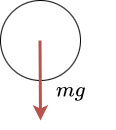
\includegraphics{source/images/newton/newton2.png}

重力のみが働く小球を考えた時,鉛直下向き方向の運動方程式は,加速度を
\(a\) とした時,

\begin{align*}
ma&=mg\\
a&=g
\end{align*}

というように,前の章で練習した内容と矛盾のない結果になるわけです.

では,運動方程式から推察できる簡単な事実を考えましょう.すなわち,力の働いていない物体はどのような運動をするのか,です.これは非常に簡単で
\(m\ddot{\boldsymbol{r}}=\boldsymbol{0},\;\dot{\boldsymbol{r}}=(\text{一定})\)
と言う非常にシンプルな結果となるわけです.つまり,次のようにまとめられるわけです.

\begin{Tbox}{定理}
ニュートンの第1法則(慣性の法則)

力の働いていない物体は,常にその速度を保つ.

\end{Tbox}

そして最後に,力の持つ性質を述べようと思います.それは,作用反作用の法則と呼ばれるものです.

\begin{Tbox}{定理}
ニュートンの第3法則(作用反作用の法則)

物体に働く力は,常にある2つの物体の間で及ぼしあうように働く.物体Aが物体Bに及ぼす力を
\(\boldsymbol{F_{BA}}\) ,物体Bが物体Aに及ぼす力を
\(\boldsymbol{F_{AB}}\) とした時,次の式が成り立つ.
\[\boldsymbol{F_{BA}}+\boldsymbol{F_{AB}}=\boldsymbol{0}\]

\end{Tbox}

つまり,地球があなたを引っ張っているのと同じくらい,あなたは地球を引っ張っているのです.非常に非直感的な法則です.同時に,壁があなたに押されていると同じくらい,あなたは壁に押されるというのも同じ作用反作用の法則です.こちらは直感的ですね.

では,具体的にはどのような力があるのでしょうか.ニュートンの発展させた古典力学という世界では,力は2種類のみです.それは,万有引力と,電磁気力です.高校で学ばれる物理の世界は,最後に学ぶ原子範囲を除き,須くこの二つの力を持ってして語り尽くされる世界で,これ以外に起因する力は一切存在し得ません.非常にシンプルですね.ただ,その力の表し方は一癖も二癖もあり,学ぶ人にとって少し難しく感じられることもあるかもしれません.

まず,重力について話をしていきましょう.重力とは,地球上の物体が地球から受ける万有引力のことです.重力の大きさは地表においてはほぼ変わらず,質量に比例した値になり,その比例係数を重力加速度といいました.ここで重要なのは,ほぼ変わらないということであり,実際には場所によって少しずつ異なる値をとります.それはなぜかという理論については,ひとまずのところ置いておいて議論を進めることになります.後々,また学ぶことになります.

次に話を避けて通れないのが,電磁気学です.電磁気学の具体的な様相についてはそれなりに高度な数学も必要で,今現状ではやらないことにしますが,少なくとも今のうちに語らなければならないことは語り尽くすことにしましょう.

我々を含む,すべての物体を,原子と呼ばれる非常に小さな粒が構成しているところは,皆さんが小中学校を通して学んだ通りであり,またその原子は中心に+に帯電した原子核,その周りにーに帯電した電子で出来上がっています.そして,その+とーは引きつけ合う性質があります.同時に,+同士やー同士では反発する性質があります.また,その力は距離が小さくなるほどに大きくなるという性質も持っています.

''塊''になっている物体内では,+とーがいい具合のバランスで固まっているのは高等学校の化学で学んだ通りであり,それらを共有結合やイオン結合などと呼んでいました.では,別々の''塊''ではどうなっているのでしょうか.それは,電子同士が非常に近い距離にまで近づき,その結果非常に大きいな反発力が働くようになるわけです.そのおかげで,私たちは,床に対して反発して立つことができるのです.そしてその,物体と物体が一体にならないように,別々の''塊''として独立して存在するように反発しあう力のことを反発力と言います.

このアイデアを次の状態で理解することにしましょう.

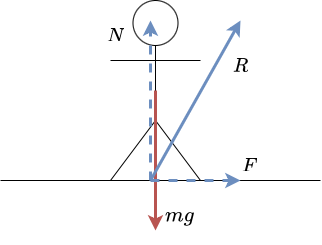
\includegraphics{source/images/newton/newton1.png}

地面に立っている人間を考えてみましょう.この人間に働く力は基本的に2種類しかなく,それは万有引力と電磁気力です.まず,地球からの万有引力である重力の
\(mg\)
があり,次に足と地面との距離が十分小さいために起きる電磁気力である反発力
\(R\) があります.この時, \(R\)
がどのような値を取るのかというのは,この時点ではまだわかりません.なぜなら,地面と人間の足の境界には
\(10^{23}\)
個程度以上の原子の周りの電子が複雑に運動しており,その様相を語り尽くすことはとてもじゃないができないからです.ですが,この人間が加速度を持っていないという前提をつけてあげることによって
\(R\) の特定ができるわけです.問題を解決しやすくするために図のように
\(R\) を \(N,F\)
に分解して,それぞれの方向に対して運動方程式を立ててやることによって

\begin{align*}
0&=mg-N\\
0&=F
\end{align*}

とのように,確定させることができるわけです.ここで, \(N,F\)
のことをそれぞれ垂直抗力,および,摩擦力と呼ばれます.

初学者にありがちなミスとして, \(mg\) があるから反発力があって \(N=mg\)
だと反射的に決めつけてしまうことがありますが,それは人が加速していない時に限るわけです.注意しましょう.

では,これらの法則を実際にどのようにして問題に応用するべきでしょうか.これからは実際に問題を解いていくことによって,それらを明らかにしていこうと思います.

\begin{Rbox}{例題}
下の図のように仰角 \(\theta\)
の斜面に物体を置いている.摩擦力がない時,この物体の持つ加速度はどうなるか.

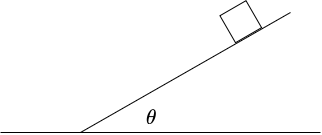
\includegraphics{source/images/newton/newton3.png}

\end{Rbox}

\tcbox[arc is angular, shrink tight, extrude by=4pt]{解答}

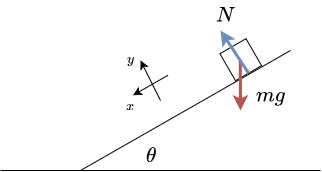
\includegraphics{source/images/newton/newton4.png}

物体と紐それぞれに対して運動方程式を立ててやると次のようになる.

\begin{align*}
m\ddot{x} &= mg \sin \theta \\
m\ddot{y} &= -mg \cos \theta + N
\end{align*}

ここで,坂自体は形を変えてしまわないので, \(y=0\)
といえて,このような,運動の様相を縛る条件を束縛条件と呼ぶ.両辺を微分することによって
\(\ddot{y}=0\) となる.

\begin{align*}
\ddot{x} &= g \sin \theta \\
N &= mg \cos \theta
\end{align*}

故に加速度の大きさは \(\sqrt{\ddot{x}^2+\ddot{y}^2}=g \sin \theta\)
で,方向は坂道の滑り落ちる方向である.

ニュートンの運動の法則は粒子に対して成り立つものであり,残念ながらある程度以上の粒子が集まっている「物体」については説明されていません.ですが,それでも,運動方程式から得られる情報はたくさんあります.例えば,とある場所に
\(n\)
個の粒子があり,それらが互いに力を及ぼしながら,外からも力を受けているとしましょう.その時,
\(i\) 番目の粒子の運動方程式は

\begin{align*}
m_i\ddot{\boldsymbol{r}_i} = \sum_j \boldsymbol{F}_{ij} +  \boldsymbol{F}_{i\text{out}}
\end{align*} ここで, \(\boldsymbol{F}_{ij}\) は \(j\) 番目の粒子が
\(i\) 番目の粒子に及ぼす力であり, \(\boldsymbol{F}_{i\text{out}}\) は
\(i\) 番目の粒子が受ける外力です.

この \(n\)
元微分方程式を解き切ることは絶望的に難しいのは簡単にわかるでしょう.ですが,全ての方程式を足し合わせることによって,
\begin{align*}
\sum_i m_i\ddot{\boldsymbol{r}_i} = \sum_i\sum_j \boldsymbol{F}_{ij} +  \sum_i\boldsymbol{F}_{i\text{out}}
\end{align*} ここで,作用反作用の法則を考えれば,
\(\sum_i\sum_j \boldsymbol{F}_{ij}=\boldsymbol{0}\) なので,
\begin{align*}
M_{\text{tot}}&=\sum_i m_i \\
\boldsymbol{r}_\text{G}&=\frac{\sum_i m_i\ddot{\boldsymbol{r}_i}}{M_{\text{tot}}}
\end{align*} と,前半で前重力,後半で加重平均(重心)を定義してやれば,
\begin{align*}
M_{\text{tot}}\ddot{\boldsymbol{r}_\text{G}} = \sum_i\boldsymbol{F}_{i\text{out}}
\end{align*}
とすることができます.これは重心(運動)方程式と呼ばれており,先の問題のように大きな物体に対して,あたかも粒子ではない物体に対しても運動方程式が当てはまるように書いているのは,重心方程式を書いているに過ぎないわけです.

以上の作業をしてみることでわかることですが,実は何に注目して運動方程式を立てるべきか,という問題に対して,内力が全て打ち消しあって,一様な外力が働いている,任意の粒子の集合部分が答えになります.何を塊として,運動方程式を立てるか,それは問題を解く人が一番やりやすい方法を選べばいいというわけですね.

\begin{Rbox}{例題}

下の図のように紐に繋がれた2つの物体があり,右側の物体を引っ張っている.紐は物体とくっついていて離れず,故に物体と紐の間には引きつけあう電磁気力である,張力が働くことに注意して,次の問いに答えよ.ただし,重力は無視し,台座は動かないものとせよ.

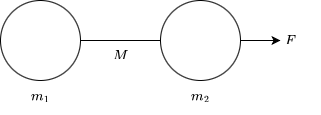
\includegraphics{source/images/newton/newton5.png}

\begin{enumerate}
\def\labelenumi{\arabic{enumi}.}
\tightlist
\item
  各物体の加速度を求めよ.
\item
  張力の大きさを求めよ.
\item
  紐の質量を無視した場合,左右の張力はどのような関係になるか.
\end{enumerate}

\end{Rbox}

\tcbox[arc is angular, shrink tight, extrude by=4pt]{解答}

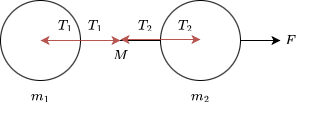
\includegraphics{source/images/newton/newton6.png}

作用反作用の法則によって張力を図のように \(T_1,\:T_2\)
と設定できる.物体それぞれに対して運動方程式を立ててやると次のようになる.
\begin{align*}
m_1a_1 &= T_1 \\
m_2a_2 &= F-T_2 \\
MA &= T_2-T_1
\end{align*}
ここで,3つの物体が同時に動くので,次のような束縛条件が科される.
\begin{align*}
a_1=a_2=A
\end{align*} 以上の条件で運動方程式を解いてしまうと \begin{align*}
a_1=a_2=A=\frac{F}{m_1+m_2+M}\\
T_1=\frac{m_1}{m_1+m_2+M}F\\
T_2=\frac{m_1+M}{m_1+m_2+M}F
\end{align*} ここで,紐の質量を \(0\) にすることで, \begin{align*}
T_1=T_2
\end{align*}
という関係がわかる.この関係は,今後も使うので注意すべし.ただし,紐の質量が無視できる場合に限ることを注意せよ.

\begin{Qbox}{問題}

下の図のように紐に繋がれた2つの物体があり,物体間には滑車がある.次の問いに答えよ.ただし,紐の質量と摩擦は無視せよ.

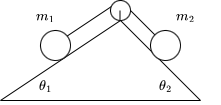
\includegraphics{source/images/newton/newton7.png}

\begin{enumerate}
\def\labelenumi{\arabic{enumi}.}
\tightlist
\item
  各物体の加速度を求めよ.
\item
  張力の大きさを求めよ.
\end{enumerate}

\end{Qbox}

\tcbox[arc is angular, shrink tight, extrude by=4pt]{解答}

\(m_1,m_2\) それぞれに働く張力の大きさを \(T_1,T_2\)
とする.右側を正としてそれぞれの斜面に沿った加速度を \(a_1,a_2\)
として,運動方程式を立てると \begin{align*}
m_1a_1=T-m_1g\sin \theta_1\\
m_2a_2=m_2g\sin \theta_2-T
\end{align*} 束縛条件は \begin{align*}
a_1=a_2
\end{align*} 解いてやれば \begin{align*}
a_1=a_2=\frac{-m_1\sin \theta_1+m_2\sin \theta_2}{m_1+m_2}g\\
T=\frac{m_1m_2}{m_1+m_2}(\sin \theta_1+\sin \theta_2)g
\end{align*}
とわかる.この問題については,脳内で次のように変換すると楽かもしれない.
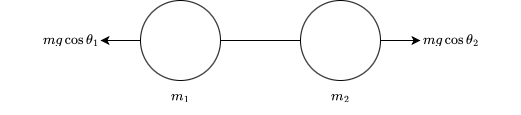
\includegraphics{source/images/newton/newton8.png}

今までの問題でも扱ってきたのですが,束縛条件にフォーカスを当てたような問題をやってみましょう.

\begin{Rbox}{例題}

下の図のように紐と滑車に繋がれた2つの物体がある.滑車の質量と摩擦力を無視して次の問題を答えよ.

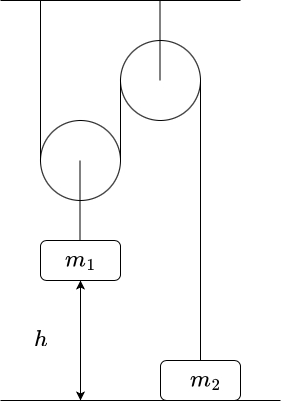
\includegraphics{source/images/newton/newton9.png}

\begin{enumerate}
\def\labelenumi{\arabic{enumi}.}
\tightlist
\item
  各物体の加速度を求めよ.
\item
  紐の張力を求めよ.
\end{enumerate}

\end{Rbox}

\tcbox[arc is angular, shrink tight, extrude by=4pt]{解答}

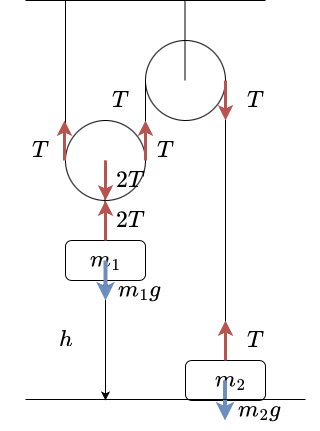
\includegraphics{source/images/newton/newton10.png}

作用反作用の法則によって張力を図のように \$T \$
と設定できる.滑車の運動方程式を考えれば,左の滑車下の張力は \(2T\)
となる.下向きを正として物体それぞれに対して運動方程式を立ててやると次のようになる.
\begin{align*}
m_1\ddot{x_1} &= m_1g-2T \\
m_2\ddot{x_2} &= m_2g-T
\end{align*} ここで,紐の長さが変わらないことから, \(m_1\)
が下がった分だけ,その倍 \(m_2\) が上がるので \begin{align*}
2\dd x_1=-\dd x_2 \\
2\ddot{x_1}+\ddot{x_2}=0
\end{align*} 以上の条件で運動方程式を解いてしまうと \begin{align*}
\ddot{x_1}=\frac{m_1-2m_2}{m_1+4m_2}g \\
\ddot{x_2}=\frac{-2m_1+4m_2}{m_1+4m_2}g \\
T=\frac{3m_1m_2}{m_1+4m_2}g
\end{align*}

\begin{Qbox}{問題}

下の図のように紐に繋がれた2つの物体があり,物体間には滑車がある.次の問いに答えよ.ただし,紐の質量と摩擦は無視し,3つの物体は離れないものとする.

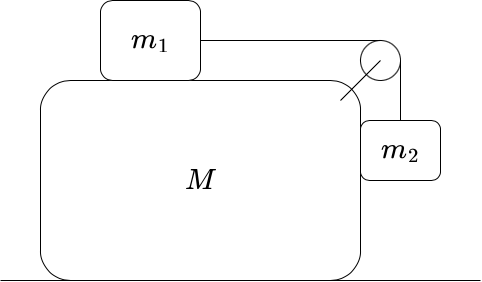
\includegraphics{source/images/newton/newton11.png}

\begin{enumerate}
\def\labelenumi{\arabic{enumi}.}
\tightlist
\item
  各物体の加速度を求めよ.
\item
  張力の大きさを求めよ.
\end{enumerate}

\end{Qbox}

\tcbox[arc is angular, shrink tight, extrude by=4pt]{解答}

\(m_1,m_2\) に働く垂直抗力を \(N_1,N_2\) として,張力を \(T\)
とする.また水平方向右を正とする \(x\) 軸,鉛直上方向を正とする \(y\)
軸を設定して運動方程式を立てる. \begin{align*}
M\ddot{X}&=-N_2-T\\
m_1\ddot{x_1} &= T \\
N_1&=m_1g\\
m_2\ddot{x_2} &= N_2\\
m_2\ddot{y_2} &=T-m_2g
\end{align*} また,束縛条件は \begin{align*}
\ddot{X}&=\ddot{x_2}\\
\ddot{x_1}-\ddot{X}&=-\ddot{y_2}
\end{align*} かなりの計算を経ることによって次のようになるとわかる.
\begin{align*}
T&=\left\{\frac{1}{M+m_2}+\frac{1}{m_1}+\frac{1}{m_2}\right\}^{-1}g\\
\ddot{X}=\ddot{x_2}&=\left\{\frac{1}{M+m_2}+\frac{1}{m_1}+\frac{1}{m_2}\right\}^{-1}\frac{g}{m_1}\\
\ddot{y_2}&=\left\{\frac{1}{M+m_2}+\frac{1}{m_1}+\frac{1}{m_2}\right\}^{-1}\frac{g}{m_2}-g
\end{align*}

\begin{Qbox}{問題}
下の図のように紐に繋がれた3つの物体があり,物体間には滑車がある.\(m_2\)
に働く張力を求めよ.ただし,紐の質量と摩擦は無視し,紐は弛まないとする.

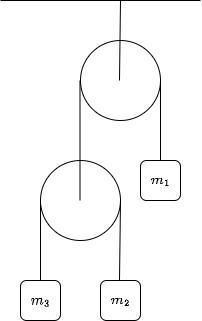
\includegraphics{source/images/newton/newton13.png}

\end{Qbox}

\tcbox[arc is angular, shrink tight, extrude by=4pt]{解答}

張力を \(T\) とする.鉛直下方向を正として運動方程式を立てる.
\begin{align*}
m_1a_1&=m_1g-2T\\
m_2a_2&=m_2g-T\\
m_3a_3&=m_3g-T
\end{align*} また,束縛条件は \begin{align*}
\ddot{x_2}+\ddot{x_3}&=-2\ddot{x_1}
\end{align*} かなりの計算を経ることによって次のようになるとわかる.
\begin{align*}
T=\left(\frac{4}{m_1}+\frac{1}{m_2}+\frac{1}{m_3}\right)^{-1}4g
\end{align*}

\begin{Qbox}{問題}
(滋賀医大)

下の図のように2つの物体がある. \(m,M\) ともに摩擦なく動くので, \(m\)
の滑り落ちる地面への角度は \(\theta\) ではなく, \(\phi\)
であるという.この時, \(\tan \phi\) を求めよ.

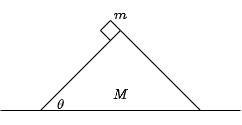
\includegraphics{source/images/newton/newton14.png}

\end{Qbox}

\tcbox[arc is angular, shrink tight, extrude by=4pt]{解答}

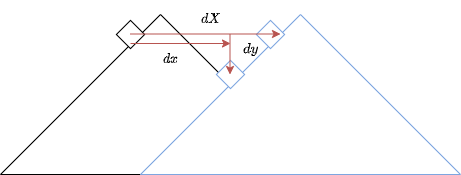
\includegraphics{source/images/newton/newton15.png}

図のように考えれば \begin{align*}
m\ddot{x}&=-N\sin\theta\\
m\ddot{y}&=mg+N\cos\theta\\
M\ddot{X}&=N\sin\theta
\end{align*} また,束縛条件は \begin{align*}
\ddot{y}=(\ddot{X}-\ddot{x})\tan\theta
\end{align*} かなりの計算を経ることによって次のようになるとわかる.
\begin{align*}
N&=\frac{mg}{1+\frac{m}{M}\sin ^2 \theta}\cos \theta\\
\tan \phi = \frac{\ddot{y}}{\ddot{x}}&=-\left(1+\frac{m}{M}\right)\tan \theta
\end{align*}
ここで,なぜ答えの値はマイナスになっているかというと,上の図のように考えているからであって,
\(\dd x\)
が右向き正だからであり,左向き正であればプラスの値が答えになる.

次に摩擦力について考えましょう.

物体と物体が''擦れる''際,その物体の動作を止めるような力が働くことは経験則で皆さん,わかることでしょう.ところが,摩擦の様相のメカニズムは非常に複雑です.すれ合う両物体の表面の原子配置は基本的に不規則であり,ある程度以上近づきあった原子同士が前に所属した物体に残留しないこともあり得るので,単純なモデル化は困難を極めます.以前は,この摩擦のメカニズムは非常に単純で,物体の表面は凹凸だらけで,その凹凸を乗り越えることで摩擦が発生すると考えられていましたが,凸凹を乗り越える際,凸凹が変形し,波動や原子運動が発生し,やがて熱が発生しますが,それでは単純な凹凸ではなく極めて複雑で時間と共に変化する凹凸を考えなくてはならなくなるのです.

ところが,摩擦力は,経験則から非常に単純な法則で近似することができます.すなわち,

\begin{align*}
F=\mu N
\end{align*}

ここで \(N\) は垂直抗力で, \(\mu\)
は摩擦係数と呼ばれる定数です.この力の特徴としては, \(F=\mu N\)
となる大きさまで物体は滑る方向に対しての力に対抗して動かずにいることができて,それ以上となると加速度を持って運動することになるというものです.また,その時,静止し続けられるまで耐えられる摩擦定数と,加速したのちの摩擦定数との値に違いがあり,前者を静止摩擦係数,後者と動摩擦係数と呼ばれます.

静止摩擦係数 \(\mu\)
を測定したい場合,傾けた斜面に物体を乗せることによって簡単に計測することができます.すなわち,物体が運動しだす瞬間では

\begin{align*}
N= mg\cos \theta \\
mg \sin \theta=\mu N
\end{align*}

との式が成り立ち, \(\mu = \tan \theta\)
と計測されるのです.動摩擦係数についても,斜面を滑り出した物体がどれほどの角度で初めてその運動を止めるかを調べることによって,同様に計測されることがわかるでしょう.

静止摩擦係数と動摩擦係数では,前者の方が大きい傾向にはあるが,乾いた金属などでは両者にほぼ差がないことがわかっています.

では,実際の問題で練習をしていきましょう.

\begin{Rbox}{例題}
下の図のように2つの物体がある.\(M\) と床,及び \(m,M\)
の間には摩擦があり, \(M\) は右向きに大きさ \(F\)
の力を受けている.この時, \(m,M\) が共に動く \(F\) と\(M\) と床,及び
\(m,M\) の間の静止摩擦係数,動摩擦係数の条件を求めよ.

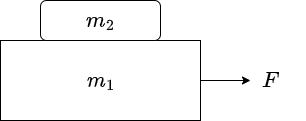
\includegraphics{source/images/newton/newton16.png}

\end{Rbox}

\tcbox[arc is angular, shrink tight, extrude by=4pt]{解答}

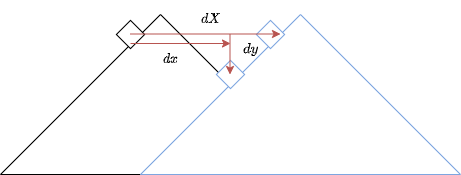
\includegraphics{source/images/newton/newton15.png}

図のように考えれば \begin{align*}
m_1a&=F-R_1-R_2\\
0&=-m_1g+N_1-N_2\\
m_2a&=R_2\\
0&=N_2-m_2g
\end{align*} この時, \(R_1\) は動摩擦力なので \(R_1=\mu _1' N_1\)
となる. \begin{align*}
R_2&=\frac{m_1m_2}{m_1+m_2}\left\{\frac{F}{m_1}-\mu_1'\left(1+\frac{m_2}{m_1}\right)\right\} \\
a&=\frac{m_1}{m_1+m_2}\left\{\frac{F}{m_1}-\mu_1'\left(1+\frac{m_2}{m_1}\right)\right\}
\end{align*} ここで同時に滑り出す条件とは \begin{align*}
a&>0\\
R_2&<\mu_2N_2
\end{align*} であるので,それらを \(F\)
についてまとめると次のようになる.
\[\mu_1(m_1+m+2)g<F \leq (\mu_1'+\mu_2)(m_1+m_2)g\]
また,ここまでの議論は \(R_2<\mu_2N_2\) を使い,それまでは具体的に
\(R_2\) を設定せずに進めたが, \(R_2=\nu_2 N_2\)
などとおいて計算を進め,最終的に \(\nu_2<\mu_2\)
とすることでも構わない.これからはどちらの方法も用いるので,混乱のないようにお願いしたい.

\begin{Qbox}{問題}

地面の上をなめらかに動くことのできる質量 \(m_1\)
の台車がある。この台車の上に,質量 \(m_2\)
のおもりを載せ,図のようにおもりに結んだロープを引いて,水平な地面上を直線コースに沿って走るレースを考える。ロープに働く張力を
\(T\) , ロープと地面のなす角を \(\theta\) , 重力加速度を \(g\)
として,以下の設問に答えよ。ただし、 \(\theta\) は与えられたものとする.

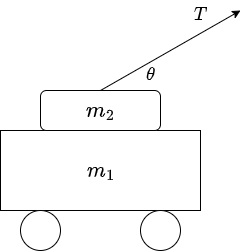
\includegraphics{source/images/newton/newton17.png}

\begin{enumerate}
\def\labelenumi{\arabic{enumi}.}
\tightlist
\item
  おもりが台車から受ける垂直抗力を求めよ.
\item
  おもりと台車の間に働く摩擦力を \(f\)
  ,台車とおもりの水平方向の加速度の大きさを \(a_1,\: a_2\)
  として,水平方向に対する台車とおもりそれぞれの運動方程式を示せ.
\item
  おもりと台車が滑ることなく一体となって動く場合,台車に与えることのできる加速度の最大値はいかほどか.台車とおもりの間の静止摩擦係数を
  \(\mu_0\) として求めよ.
\item
  上記の範囲内の加速度を出すことはできるが,速さ \(v_0\)
  よりは早く走ることのできない人が,おもりと台車の間で滑りを起こすことなく台車を引いて最も速くゴールに到達することを考える。スタートからゴールまで,加速度
  \(a\) ,速度 \(v\) で,走行距離 \(s\) をそれぞれ時間 \(t\)
  に対してどのように変化させればよいか. \(a,\:v,\: s\) を \(t\)
  の関数として求め,図示せよ.ただし,ゴールまでの距離 \(s_0\) は
  \(v_0^2/a_0\) とする
\end{enumerate}

\end{Qbox}

\tcbox[arc is angular, shrink tight, extrude by=4pt]{解答}

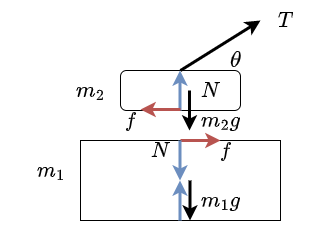
\includegraphics{source/images/newton/newton18.png}

図のように考えれば \begin{align*}
N&=m_2g-T\sin\theta\\
m_1a_1&=f\\
m_2a_2&=T\cos\theta-f
\end{align*} また,束縛条件は \begin{align*}
a_1=a_2:=a
\end{align*} 計算を経ることによって次のようになるとわかる.
\begin{align*}
a&=\frac{T}{m_1+m_2}\cos\theta\\
f&=\frac{m_1}{m_1+m_2}T\cos\theta
\end{align*} 以上で問題1,2はは完了した.

3.ここで \(f<\mu_0 N\) が求める条件なので, \begin{align*}
a\leq \frac{\mu_0m_2g}{m_1+\mu_0(m_1+m_2)\tan \theta}
\end{align*} となる.

4.加速度が常に最大になるように動けばいいことは明らかである.つまり,速さ
\(v_0\) に達するまで加速度 \(a_0\)
で動き,その後は等速でゴールまで辿り着くということである.つまり
\(v_0/a_0=t_0,\; 3v_0/2a_0 =t_1\)
として(それぞれ,加速を止める時刻とゴールする時刻である)

\begin{align*}
a=a_0,\;v=a_0t,\;s=\frac{1}{2}a_0t^2\;(0\leq t \leq t_0) \\
a=0,\;v=v_0,\;s=\frac{v_0^2}{2a_0} + v_0(t-t_0)\;(t_0\leq t \leq t_1)
\end{align*}

\begin{Qbox}{問題}
下の図のように動かない角度が \(\theta\) の斜面に,2つの
\textbf{互いに接している}
物体がある.両物体と斜面の静止摩擦係数,動摩擦係数はそれぞれ等しく,それぞれ
\(m_1,\:m_2\) に関して \(\mu _1,\:\mu _2\) となっている.ただし
\(\mu_1>\mu_2\) である.この時

\begin{enumerate}
\def\labelenumi{\arabic{enumi}.}
\tightlist
\item
  両物体が共に滑り落ちている時,物体間に働く抗力の大きさを求めよ.
\item
  両物体が滑らないで済む斜面の角度の最大値を求めよ.
\end{enumerate}

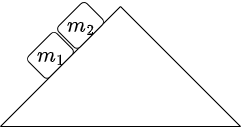
\includegraphics{source/images/newton/newton19.png}

\end{Qbox}

\tcbox[arc is angular, shrink tight, extrude by=4pt]{解答}

斜面下向きに沿った座標軸を考え,物体の加速度を \(a\)
,物体同士に働く抗力の大きさを \(N\) ,とした時次のようになる.
\begin{align*}
m_1a&=m_1g\sin \theta -\mu_1m_1g\cos \theta +N\\
m_2a&=m_2g\sin \theta -\mu_1m_1g\cos \theta -N
\end{align*} 連立方程式を解くことによって次のようになるとわかる.
\begin{align*}
a&=g\sin \theta - g \cos \theta \frac{\mu_1m_1+\mu_2m_2}{m_1+m_2}
N&=\frac{m_1m_2}{m_1+m_2}(\mu_1-\mu_2)g\cos\theta
\end{align*} ここで滑らないで済むということは \(a=0\) ということなので,
\begin{align*}
\tan \theta = \frac{\mu_1m_1+\mu_2m_2}{m_1+m_2}
\end{align*} というのが滑らない限界の大きさの角である.

\begin{Qbox}{問題}
(東京大)

下図のように水平面に対して \(45^{\circ}\) の角度をなす斜面上に質量 \(M\)
の直角二等辺三角形の物体Aを斜辺の面が斜面と接するように置く.直角二等辺三角形の等しい2辺の長さをdとする.Aの上面に質量
\(m\) で,大きさの無視できる小さな物体Bを置く。斜面上に原点 \(O\)
をとり,水平右向きに \(x\) 軸,鉛直下向きに \(y\)
軸をとる.はじめ,Aは上面が \(y=0\)
となる位置にあり,BはAの上面の右端,すなわち \((x,\:y)=(d,\:0)\)
の位置にある.空気の抵抗および斜面とAの間の摩擦は無視できるものとし,重力加速度を
\(g\) とする。

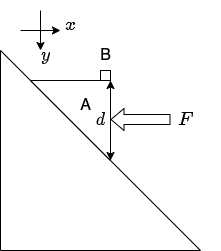
\includegraphics{source/images/newton/newton23.png}

I AとBの間の摩擦も無視できる場合に以下の問いに答えよ.

\begin{enumerate}
\def\labelenumi{\arabic{enumi}.}
\tightlist
\item
  図のようにAの右面に水平左向きに力 \(F\)
  を加えたところ,2つの物体は最初の位置に静上したままであった. \(F\)
  の大きさを求めよ.
\item
  力 \(F\)
  を取り除いたところ,AとBは運動を開始した.その後,BはA上面の左端に達した.この瞬間のBの
  \(y\) 座標を求めよ.
\item
  BがA上面の左端に達する直前のBの速さ \(v\) を求めよ.
\end{enumerate}

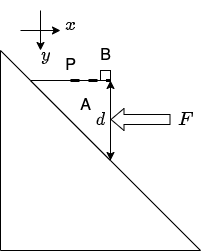
\includegraphics{source/images/newton/newton21.png}

Ⅱ 図1-2に示すようにA上面の点Pを境にして右側の表面が粗く,この部分での
AとBの間の静止摩擦係数および動摩擦係数はそれぞれ \(\mu,\:\mu'\) (ただし
\(\mu > \mu'\) )
である.A上面の点Pより左側は,なめらかなままである・問I1と同様に,力
\(F\) を加えて両物体を静止させた.力 \(F\)
を取り除いた後の両物体の運動について以下の間に答えよ.

\begin{enumerate}
\def\labelenumi{\arabic{enumi}.}
\tightlist
\item
  \(\mu\)
  が十分に大きい場合,BはA上面を滑り出さず,両物体は一体となって斜面を滑りおりる.このときの両物体の
  \(x\) 方向の加速度 \(a_x\) と \(y\) 方向の加速度 \(a_y\) を求めよ.
\item
  \(\mu\) がある値 \(\mu_0\)
  より大きければBはA上面を滑り出さず,小さければ滑り出す.その値
  \(\mu_0\) を求めよ.
\item
  \(\mu\) が \(\mu_0\) より小さい場合に,Bが最初の位置
  \((x,\:y)=(d,\:0)\)
  からA上面の左端に達するまでの運動の様相を述べた次の文章の空欄に語群から適切な言葉を選び入れよ.
\end{enumerate}

最初物体が点Bと点Pの間にあるうちは(ア)運動をしており,その後は(イ)運動をする.

語群:等速,等加速度

\end{Qbox}

\tcbox[arc is angular, shrink tight, extrude by=4pt]{解答}

I

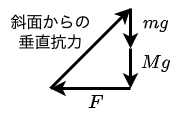
\includegraphics{source/images/newton/newton24.png}

\begin{enumerate}
\def\labelenumi{\arabic{enumi}.}
\tightlist
\item
  上図の通り, \(F=(m+M)g\)
\item
  \(y=d\)
\item
  \(m,\:M\) の加速度の大きさを \(a,\:A\) ,物体間の垂直抗力を \(N\)
  として運動方程式を立てれば次のようになる. \begin{align*}
  ma&=mg-N\\
  MA&=\frac{Mg+N}{\sqrt{2}}\\
  \sqrt{2}a&=A
  \end{align*} これを解いてやれば \begin{align*}
  a=\frac{m+M}{m+2M}g
  \end{align*} ここで,等加速度運動なので \begin{align*}
  v=\sqrt{2ad}=\sqrt{2gd\frac{M+m}{2M+m}}
  \end{align*}
\end{enumerate}

Ⅱ

\begin{enumerate}
\def\labelenumi{\arabic{enumi}.}
\tightlist
\item
  両物体の加速度を \(a\) として運動方程式を立てれば次のようになる.
  \begin{align*}
  (M+m)a=\frac{M+m}{\sqrt{2}}g\\
  \end{align*} 以上から \begin{align*}
  a_x=a_y=\frac{1}{\sqrt{2}}a=\frac{1}{2}g
  \end{align*}
\item
  摩擦力と垂直抗力を \(R,\:N\)
  とすれば小物体の運動方程式は次のようになる. \begin{align*}
  ma_x&=R\\
  ma_y&=mg-N
  \end{align*} 上の結果と合わせれば \(R/N=1=\mu_0\) とわかる.
\item
  点Pを境にその前では(ア)等加速度運動であり,その後は(イ)等速運動である.
\end{enumerate}

\begin{Qbox}{問題}
質量 \(m\) の物体が重力と抵抗力を受けて鉛直下向きに速度 \(v\)
で落下している.抵抗力の大きさは物体の速さに比例すると仮定し,比例定数を
\(k\) とする.また,速度とか速度は鉛直下向きを正にとる.物体の位置を
\(x\)
とすると,この物体の運動方程式はどうなるか.また,物体の速さを時間の関数として求め,十分時間経った時の速さ(終端速度)を求めよ.

\end{Qbox}

\tcbox[arc is angular, shrink tight, extrude by=4pt]{解答}

\begin{align*}
m\ddot{x}&=mg-k\dot{x}\\
\dot{x} &= \frac{mg}{k}\left(1-e^{-\frac{k}{m}t}\right)
\end{align*} 終端速度は \(mg/k\) である.

\bookmarksetup{startatroot}

\hypertarget{ux904bux52d5ux91cfux904bux52d5ux30a8ux30cdux30ebux30aeux30fcux3068ux4ed5ux4e8buxff12ux4f53ux554fux984c}{%
\chapter{運動量,運動エネルギーと仕事,2体問題}\label{ux904bux52d5ux91cfux904bux52d5ux30a8ux30cdux30ebux30aeux30fcux3068ux4ed5ux4e8buxff12ux4f53ux554fux984c}}

\hypertarget{ux904bux52d5ux91cf}{%
\section{運動量}\label{ux904bux52d5ux91cf}}

運動方程式はそれ単体でかなりの現象を説明するものですが,世の中にはあまりにも多くの粒子が複雑に互いに力を及ぼし合っているので,解析し切ることができることが難しいことが多いです.

そんな中で,前章でも述べた通り,多粒子を考える方法はあり,これからはその方法の一つを考えることにしましょう.

まず,言葉の定義として,運動量について紹介します.

\begin{Dbox}{定義}
とある物体が質量 \(m\) ,速度 \(\boldsymbol{v}\)
を持っている時,その物体の運動量 \(\boldsymbol{p}\)
を次のように定義する.

\[\boldsymbol{p}=m\boldsymbol{v}\]

\end{Dbox}

つまり,運動方程式は次のようにかけます.
\[\dot{\boldsymbol{p}}=\boldsymbol{F}\]
多粒子系について考えましょう.前章と同様,とある場所に \(n\)
個の粒子があり,それらが互いに力を及ぼしながら,外からも力を受けているとしましょう.その時,
\(i\) 番目の粒子の運動方程式は \begin{align*}
\dot{\boldsymbol{p}_i} = \sum_j \boldsymbol{F}_{ij} +  \boldsymbol{F}_{i\text{out}}
\end{align*} ここで, \(\boldsymbol{F}_{ij}\) は \(j\) 番目の粒子が
\(i\) 番目の粒子に及ぼす力であり, \(\boldsymbol{F}_{i\text{out}}\) は
\(i\) 番目の粒子が受ける外力です.この式を全ての \(i\)
について足し合わせることによって, \begin{align*}
\sum_i \dot{\boldsymbol{p}_i} &= \sum_i\sum_j \boldsymbol{F}_{ij} +  \sum_i\boldsymbol{F}_{i\text{out}}
\end{align*} 作用反作用の法則によって,
\(\sum_i\sum_j \boldsymbol{F}_{ij}\) となるので, \begin{align*}
\sum_i \dot{\boldsymbol{p}_i} &= \sum_i\boldsymbol{F}_{i\text{out}}
\end{align*} ここで外力がないとすると, \begin{align*}
\sum_i \dot{\boldsymbol{p}_i} &= \boldsymbol{0}\\
\dv{t}\sum_i \boldsymbol{p}_i &= \boldsymbol{0}\\
\sum_i \boldsymbol{p}_i &= \textbf{Const.}=M_{\text{tot}}\dot{\boldsymbol{r}}_{\text{G}}
\end{align*}
このような結果が得られるわけです.このようにある値が定数であり続けることを,値が保存していると呼ばれます.また,全運動量の合計は,全質量と重心速度の積によって表すことができることもわかりました.以上をまとめると,

\{.Tbox data-latex=``\{定理\}''\}

外力の働かない系では,全運動量が保存する.また,系の全運動量 \(\vb*{P}\)
は

\[\vb*{P}=M_{\text{tot}}\boldsymbol{v}_{\text{G}} \]

で表すことができる. :::

ここで,重心の定義を考えた時, \begin{align*}
\sum_i m_i (\boldsymbol{r}_i-\boldsymbol{r}_\text{G})=\sum_i m_i \boldsymbol{r}_{i\text{G}}=\vb*{P}_{\text{in}}=\boldsymbol{0}
\end{align*}

ここで, \(\vb*{P}_{\text{in}}\)
重心から見た物体内部の全運動量ということで,内部運動量と呼ばれています.つまり,

::: \{.Tbox data-latex=``\{定理\}''\} 定理

任意の系を,重心を原点とする座標系で見れば,全運動量は
\(\boldsymbol{0}\) となる.別の言い方をすれば,内部運動量は常に
\(\boldsymbol{0}\) となる.

:::

\begin{Rbox}{例題}
宇宙の外力の及ばない場所に星がひとつあった.その星の中で何らかの現象が起き,その結果,二つの星が出来上がり,片方は質量
\(m_1\) で速度 \(\boldsymbol{v_1}\) だった.もう片方の質量が \(m_2\)
だった時の速度を求めよ.

\end{Rbox}

\tcbox[arc is angular, shrink tight, extrude by=4pt]{解答}

\[m_1\boldsymbol{v_1}+m_2\boldsymbol{v_2}=\boldsymbol{0}\]
\[\boldsymbol{v_2}=-\frac{m_1}{m_2}\boldsymbol{v_1}\]

\hypertarget{ux904bux52d5ux30a8ux30cdux30ebux30aeux30fc}{%
\section{運動エネルギー}\label{ux904bux52d5ux30a8ux30cdux30ebux30aeux30fc}}

運動方程式の両辺に \(\vb*{v}\) を内積でかけてやることによって,
\[m\dot{\boldsymbol{v}}\cdot \boldsymbol{v}=\boldsymbol{F}\cdot\vb*{v}\]
この左辺は,
\[m\dot{\boldsymbol{v}}\cdot \boldsymbol{v}=\dv{t}\left(\frac{1}{2}m\boldsymbol{v}\cdot \boldsymbol{v}\right)=\dv{t}\left(\frac{1}{2}mv^2\right)\]
と計算されるので,
\[\dv{t}\left(\frac{1}{2}mv^2\right)=\boldsymbol{F}\cdot\vb*{v}\]
ここで,左辺の被微分部分の \(mv^2/2\)
は物体の運動エネルギーと呼ばれ,右辺は仕事率と呼ばれています.

両辺を \(t=t_0\) から \(t=t_1\)
で積分してやれば,それぞれの時刻における速度や位置を
\(\vb*{v_0},\:\vb*{v_1},\:\vb*{r_0},\:\vb*{r_1}\) などとおけば,
\begin{align*}
\frac{1}{2}mv_1^2-\frac{1}{2}mv_2^2&=\int_{t_0}^{t_1}\boldsymbol{F}\cdot\vb*{v}\dd{t}\\
&=\int_{t_0}^{t_1}\boldsymbol{F}\cdot\dv{\vb*{r}}{t}\dd{t}\\
&=\int_{\vb*{r}_0}^{\vb*{r}_1}\boldsymbol{F}\cdot \dd{\vb*{r}}
\end{align*}
この式の右辺は仕事と呼ばれています.以上のことをまとめると次のようになります.

::: \{.Tbox data-latex=``\{定理\}''\} 法則

\begin{align*}
\frac{1}{2}mv_1^2-\frac{1}{2}mv_2^2&=\int_{\vb*{r}_0}^{\vb*{r}_1}\boldsymbol{F}\cdot \dd{\vb*{r}}
\end{align*}
上式の示す通り,運動エネルギーの変化の値は,仕事の値と等しい.

:::

では,実際にこの法則に従って,問題を解いてみることにしましょう.

\begin{Rbox}{例題}
鉛直下向きに速さ \(v_1\) の物体が,高さ \(d\)
だけ落下した.この時の物体の速さを求めよ.

\end{Rbox}

\tcbox[arc is angular, shrink tight, extrude by=4pt]{解答}

\begin{align*}
\frac{1}{2}mv_1^2-\frac{1}{2}mv_2^2&=\int_{y_0}^{y_1}mg \dd{y} = mg(y_1-y_0) = mgd\\
v_2=\sqrt{v_1^2+2gd}
\end{align*}

この問題は,運動方程式を解いてやれば解決するものです.ですが,その場合,物体の座標を時間の関数で表すことになるので,労力は大きく変わるでしょう.
\[v^2-v_0^2=2\int a \dd{x}\]
この式を使うと似たようなことができると気付いた方もいらっしゃるかもしれません.ですがこの式は実質的にエネルギーの式と同等なのです.前に導出した時と導出方法は少しばかり違うのですが,どちらの方法もできるようになりましょう.

では,運動量と同様に多粒子系での運動エネルギーの様相を見てみましょう.

\[\dv{t}\left(\frac{1}{2}mv_i^2\right)=\dv{K_i}{t}=\dot{K}_i=\sum_j \boldsymbol{F}_{ij}\cdot\vb*{v}_i+\boldsymbol{F}_{i\text{out}}\cdot\vb*{v}_i\]
\[\sum_i \dot{K}_i=\sum_i\sum_j \boldsymbol{F}_{ij}\cdot\vb*{v}_i(=P_{\text{in}})+\sum_i\boldsymbol{F}_{i\text{out}}\cdot\vb*{v}_i(=P_{\text{out}})\]
ここで, \(P_{\text{in}},\:P_{\text{out}}\)
はそれぞれ,内力による仕事率と外力による仕事率です.仕事率(Power)は運動量とは違うので注意してください.
\begin{align*}
P_{\text{in}}=\sum_i\sum_j \boldsymbol{F}_{ij}\cdot\vb*{v}_i
\end{align*} \begin{align*}
\boldsymbol{F}_{ij}\cdot\vb*{v}_i+\boldsymbol{F}_{ji}\cdot\vb*{v}_j&=\boldsymbol{F}_{ij}\cdot\vb*{v}_i-\boldsymbol{F}_{ij}\cdot\vb*{v}_j\\
&=\boldsymbol{F}_{ij}\cdot(\boldsymbol{v}_{i}-\boldsymbol{v}_{j})=\boldsymbol{F}_{ij}\cdot\boldsymbol{v}_{ij}
\end{align*} なので, \[
P_{\text{in}}=\sum_i\sum_j \boldsymbol{F}_{ij}\cdot\vb*{v}_i=\sum_{i<j}\boldsymbol{F}_{ij}\cdot\boldsymbol{v}_{ij}
\] この時, \(P_{\text{out}}=0\)
つまり,外力が仕事をしなければ,粒子間の相互作用の力による仕事率は,それらの相対運動で求めたものとなるのです.

同時に,粒子間の相互作用による力,つまり,内力によっては重心速度が変わらないことは,運動量の

この詳細については2体運動を説明する際に深掘り,再びこのトピックに戻って語ることになるので,今は法則としてだけまとめることとします.

::: \{.Tbox data-latex=``\{定理\}''\} 法則

\[\dot{K}=\sum_{i<j}\boldsymbol{F}_{ij}\cdot\boldsymbol{v}_{ij}\]

系全体の運動エネルギー変化は,外力の仕事が \(0\)
の場合,粒子間の相互作用の力による仕事のみによって決定され,それらの相対運動で求めたものとなる.

:::

ここで注意しなければならないのは,系の内部運動は系の重心運動に対して影響を与えないことです.それは,系の全運動量は外力によってのみ変化し,全運動量の式
\[\vb*{P}=M_{\text{tot}}\boldsymbol{v}_{\text{G}} \]
を考えれば,重心速度の変化はないことから理解されます.

次に \(P_{\text{out}}\)
について考察すると,これはシンプルに外力が重心運動に対してなす仕事率と重心から見た内部運動に対してなす仕事率によって分解することができます.

\begin{align*}
P_{\text{out}} &= \sum_i\boldsymbol{F}_{i\text{out}}\cdot\vb*{v}_i\\
&= \sum_i\boldsymbol{F}_{i\text{out}}\cdot(\vb*{v}_{\text{G}}+\vb*{v}_{i\text{G}})\\
&=\sum_i\boldsymbol{F}_{i\text{out}}\cdot\vb*{v}_{\text{G}}+\sum_i\boldsymbol{F}_{i\text{out}}\cdot\vb*{v}_{i\text{G}}
\end{align*}

この分解の意味は,全運動エネルギー変化の \(\sum_i \dot{K}_i\)
の分解によって意味が生まれます.

\begin{align*}
K&=\sum_i K_i=\sum_i\left(\frac{1}{2} m_iv_i^2\right)=\sum_i\left(\frac{1}{2} m_i|\vb*{v}_{\text{G}}+\vb*{v}_{i\text{G}}|^2\right)\\
&= \frac{1}{2}\left(\sum_im_i\right)v_{\text{G}}^2+\sum_i\left(\frac{1}{2} m_iv_{i\text{G}}^2\right)+\sum_im_i\vb*{v}_{\text{G}}\cdot \vb*{v}_{i\text{G}}
\end{align*}

ここで前に法則とした,
\(\sum_i m_i\boldsymbol{r}_{i\text{G}}=\boldsymbol{0}\) を考えれば,

\begin{align*}
K&=\frac{1}{2}M_{\text{tot}}v_{\text{G}}^2+\sum_i\left(\frac{1}{2} m_iv_{i\text{G}}^2\right)\\
&=K_{\text{G}}+K_{\text{in}}
\end{align*}

と分解ができます.前の項を重心運動エネルギー,後ろの項を内部運動エネルギーと呼びます.ここで,

\begin{align*}
\dot{\vb*{P}}=\sum_i \dot{\boldsymbol{p}_i} &= \sum_i\boldsymbol{F}_{i\text{out}}\\
&=M_{\text{tot}}\boldsymbol{v}_{\text{G}} 
\end{align*} と言う式を思い出していただければ, \begin{align*}
M_{\text{tot}}\dot{\boldsymbol{v}}_{\text{G}}&=\sum_i\boldsymbol{F}_{i\text{out}}\\
M_{\text{tot}}\dot{\boldsymbol{v}}_{\text{G}}\cdot \boldsymbol{v}_{\text{G}}&=\sum_i\boldsymbol{F}_{i\text{out}}\cdot \boldsymbol{v}_{\text{G}}\\
\dv{t}\left(\frac{1}{2}M_{\text{tot}}v_{\text{G}}^2 \right)&=\sum_i\boldsymbol{F}_{i\text{out}}\cdot \boldsymbol{v}_{\text{G}}\\
\dot{K_{\text{G}}}&=\sum_i\boldsymbol{F}_{i\text{out}}\cdot \boldsymbol{v}_{\text{G}}
\end{align*}

この式の表す意味とは,重心運動エネルギーを変化させているのは,外力のみであり,内力は重心運動エネルギーを変化させないことです.つまり,ある系,例えば宇宙で孤立している星などを考えれば,内部でどんな大爆発が起きて粉々に砕け散ろうとも,重心運動エネルギーは変化しないのです.逆に,

\[
\dot{K_{\text{in}}}=\sum_{i<j}\boldsymbol{F}_{ij}\cdot\boldsymbol{v}_{ij}+\sum_i\boldsymbol{F}_{i\text{out}}\cdot\vb*{v}_{i\text{G}}
\]

となるために,内部運動エネルギーは内力の影響のみならず,外力からの影響を受けることになるわけです.

これまでの事実をまとめると以下のようになるわけです.

\begin{longtable}[]{@{}
  >{\raggedright\arraybackslash}p{(\columnwidth - 8\tabcolsep) * \real{0.2000}}
  >{\raggedright\arraybackslash}p{(\columnwidth - 8\tabcolsep) * \real{0.2000}}
  >{\raggedright\arraybackslash}p{(\columnwidth - 8\tabcolsep) * \real{0.2000}}
  >{\raggedright\arraybackslash}p{(\columnwidth - 8\tabcolsep) * \real{0.2000}}
  >{\raggedright\arraybackslash}p{(\columnwidth - 8\tabcolsep) * \real{0.2000}}@{}}
\toprule\noalign{}
\begin{minipage}[b]{\linewidth}\raggedright
状態
\end{minipage} & \begin{minipage}[b]{\linewidth}\raggedright
全部運動量
\end{minipage} & \begin{minipage}[b]{\linewidth}\raggedright
内部運動量
\end{minipage} & \begin{minipage}[b]{\linewidth}\raggedright
重心運動エネルギー
\end{minipage} & \begin{minipage}[b]{\linewidth}\raggedright
内部運動エネルギー
\end{minipage} \\
\midrule\noalign{}
\endhead
\bottomrule\noalign{}
\endlastfoot
立式 & \(\vb*{P}=M_{\text{tot}}\boldsymbol{v}_{\text{G}} \) &
\(\vb*{P}_{\text{in}}=\sum_i m_i \boldsymbol{r}_{i\text{G}}(=\boldsymbol{0})\)
& \(K_{\text{G}}=\frac{1}{2}M_{\text{tot}}v_{\text{G}}^2\) &
\(K_{\text{in}}=\sum_i\left(\frac{1}{2} m_iv_{i\text{G}}^2\right)\) \\
外力が働く & \(\dot{\vb*{P}}=\sum_i\boldsymbol{F}_{i\text{out}}\) &
\(\dot{\vb*{P}}_{\text{in}}=\vb*{0}\) &
\(\dot{K}_{\text{G}}=\sum_i\boldsymbol{F}_{i\text{out}}\cdot \boldsymbol{v}_{\text{G}}\)
&
\(\dot{K}_{\text{in}}=\sum_{i<j}\boldsymbol{F}_{ij}\cdot\boldsymbol{v}_{ij}+\sum_i\boldsymbol{F}_{i\text{out}}\cdot\vb*{v}_{i\text{G}}\) \\
説明 & 運動方程式をすべて足し合わせただけである & 内部運動量は常に
\(\vb*{0}\) であり,ゆえに重心速度も同じである &
内部運動は重心運動エネルギーに働きかけないので,外力による仕事率のみ考えている
&
相対運動の仕事率と,外力による内部運動エネルギーへ働きかける仕事率を考えなければならない \\
外力が働かない & \(\dot{\vb*{P}}=\vb*{0}\) &
\(\dot{\vb*{P}}_{\text{in}}=\vb*{0}\) & \(\dot{K}_{\text{G}}=0\) &
\(\dot{K}_{\text{in}}=\sum_{i<j}\boldsymbol{F}_{ij}\cdot\boldsymbol{v}_{ij}\) \\
説明 & 外力が働かないので,運動方程式から明らかに変化がない &
内部運動量は常に \(\vb*{0}\) &
外力が働かないので,重心に働きかける仕事率がない &
外力が働かない時は全運動エネルギーは内部運動エネルギーのみであり,その変化は相対運動の仕事率によって決定される \\
\end{longtable}

以上の事実は角運動量に対しても整理しておくと良いのですが,それは後に回すことにしましょう.まずは,これらの事実をふんだんに使う高校物理の花形である2体問題について考え,それに慣れましょう.まだまだ説明が続きますが,もう少しの辛抱です!

\hypertarget{ux4f53ux554fux984c}{%
\section{2体問題}\label{ux4f53ux554fux984c}}

とある孤立した(外力の働かない) \(n\)
個の粒子に対して運動方程式を立ててみることにしましょう.

\begin{align*}
\sum_i \dot{\boldsymbol{p}_i} &= \sum_i\sum_j \boldsymbol{F}_{ij}
\end{align*}

この数式において,未知数はどれだけあるでしょうか.当然ですが,各粒子の加速度と位置なので,
\(6n\) 個あるわけです.ですが,方程式の数は \(3n\)
個しかないのです.なので, \(n\)
個の粒子に対しての運動方程式を解き切ることが昔から知られています.

\tcbox[arc is angular, shrink tight, extrude by=4pt]{解答}

物事は実はこんなに簡単なわけではなく,解析力学などの知識を駆使して初めてわかるものです.ここではこれ以上深く立ち入らないために,誤魔化した話し方をしています.気になるからは,自ら調べてみるといいかもしれません.

ところが,1体問題は単純な微分方程式であり,ゆえに高校で学ぶ程度の解析学の知識を使えばどうにかなる問題が多かったですね.実は2体問題に対しても,同じことが言えるのです.それは,2体問題の持つ数学的な特性によるものが大きく,3体問題に対しては使うことができないものです.

皆さんが解くことになる入試問題の大半はこの2体問題に関するものになります.

では,実際に2体問題について考えていきましょう.

\begin{align*}
m_1 \ddot{\boldsymbol{r}_1} &= \boldsymbol{F}_{12} +\boldsymbol{F}_{1\text{out}}\\
m_2 \ddot{\boldsymbol{x}_2} &= \boldsymbol{F}_{21} +\boldsymbol{F}_{2\text{out}}
\end{align*}

これらの式を足し合わせることによって,2物体を1物体として看做したような,重心運動方程式ができるのは,皆さんがすでに学んだことですね.

\begin{align*}
M_{\text{tot}} \ddot{\boldsymbol{r}_{\text{G}}} = \boldsymbol{F}_{1\text{out}}+\boldsymbol{F}_{2\text{out}}
\end{align*}

ここで,二つの運動方程式を両辺その質量で割ったのちに差をとってみることにしましょう.

\begin{align*}
\ddot{\boldsymbol{r}_1}-\ddot{\boldsymbol{r}_2} = \left(\frac{1}{m_1}+\frac{1}{m_2}\right) \boldsymbol{F}_{12}+\frac{\boldsymbol{F}_{1\text{out}}}{m_1}-\frac{\boldsymbol{F}_{2\text{out}}}{m_2}
\end{align*} この式を運動方程式のようにまとめると, \begin{align*}
\frac{m_1m_2}{m_1+m_2}\ddot{\boldsymbol{r}_{12}}=\mu\ddot{\boldsymbol{r}_{12}}=\boldsymbol{F}_{12} +\frac{m_2\boldsymbol{F}_{1\text{out}}-m_1\boldsymbol{F}_{2\text{out}}}{m_1+m_2}
\end{align*} ここで, \(\boldsymbol{F}_{12}\) が \(\boldsymbol{r}_{12}\)
の関数であることを思い出せば,この運動方程式はあたかも1体問題の運動方程式と同等に見えるのではないでしょうか.そして,この運動方程式は相対運動を見た運動方程式ということで,相対運動方程式と呼ばれます.また特に
\(\mu = \dfrac{m_1m_2}{m_1+m_2}\) のことを換算質量と呼びます.

つまり,今までやってきたことをまとめると,2体問題の運動方程式は,重心運動方程式と相対運動方程式に分けることができ,それらは1体問題と同じ形をしているので,解き切ることができるわけです.

ここでも重心から物事を見ることの大事さがわかるでしょう.

次に,2体問題の持つ特徴についてまとめてみましょう,

\begin{equation*}
\left\{ \,
    \begin{aligned}
    & \boldsymbol{r}_{1\text{G}}=\boldsymbol{r}_1-\boldsymbol{r}_{\text{G}}=\frac{m_2}{m_1+m_2}\boldsymbol{r}_{12} \\
    & \boldsymbol{r}_{1\text{G}}=\boldsymbol{r}_1-\boldsymbol{r}_{\text{G}}=-\frac{m_1}{m_1+m_2}\boldsymbol{r}_{12}
    \end{aligned}
\right.
\end{equation*}

両辺を時間で微分すれば

\begin{equation*}
\left\{ \,
    \begin{aligned}
    & \boldsymbol{v}_{1\text{G}}=\boldsymbol{v}_1-\boldsymbol{v}_{\text{G}}=\frac{m_2}{m_1+m_2}\boldsymbol{v}_{12} \\
    & \boldsymbol{v}_{1\text{G}}=\boldsymbol{v}_1-\boldsymbol{v}_{\text{G}}=-\frac{m_1}{m_1+m_2}\boldsymbol{v}_{12}
    \end{aligned}
\right.
\end{equation*}

以上のことをまとめれば,

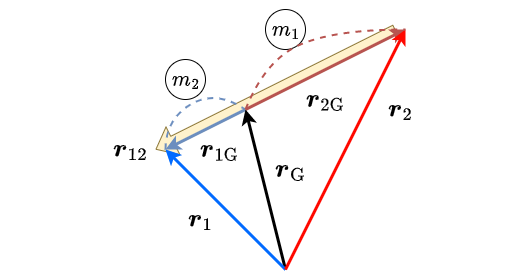
\includegraphics{source/images/energy/energy2.png}

::: \{.Tbox data-latex=``\{定理\}''\} 法則

重心系から見た2物体までの距離は質量の逆比で決まり,速さについても同じである.

:::

また,全運動量は前に確認した通り,
\[\vb*{P}=M_{\text{tot}}\boldsymbol{v}_{\text{G}} \]
であり,運動エネルギーを重心運動エネルギーと内部運動エネルギーについて分解すると,
\begin{align*}
K_{\text{G}}&=\frac{1}{2}M_{\text{tot}}v_{\text{G}}^2\\
K_{\text{in}}&=\sum_i\left(\frac{1}{2} m_iv_{i\text{G}}^2\right)=\frac{1}{2}\frac{m_1m_2}{m_1+m_2}v_{12}^2=\frac{1}{2}\mu v_{12}^2
\end{align*}
となることがわかります.この時,内部運動エネルギーを相対運動エネルギーと呼ぶこともあります.特に,外力の働かない状態では
\(\dot{K}_{\text{G}}=0,\;\dot{K}_{\text{in}}=\sum_{i<j}\boldsymbol{F}_{ij}\cdot\boldsymbol{v}_{ij}\)
だったことを思い出していただければ,
\[\dot{K}_{\text{all}}=\boldsymbol{F}_{12}\cdot\boldsymbol{v}_{12}\]
\[\Delta K_{\text{all}} = \int \boldsymbol{F}_{12}\cdot\boldsymbol{v}_{12}\dd t = \int \boldsymbol{F}_{12}\cdot\dd{\boldsymbol{r}_{12}}\]

とわかるでしょう.ではこれらの事実を確認するために,問題を解いていきましょう.

\begin{Rbox}{例題}

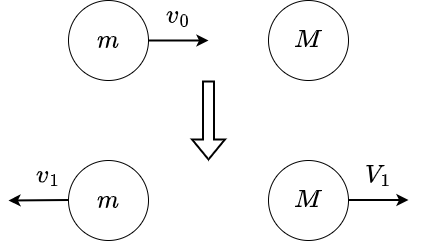
\includegraphics{source/images/energy/energy3.png}

宇宙に2物体 \(m,M\)
があり,それらはお互い退け合う力(斥力)が働く.最初( \(t=0\) ), \(m\)
が真っ直ぐ \(M\) に向かって速さ \(v_0\)
で進入していたが,斥力のために,最終的には \(m\)
は最初の速度の方向とは逆向きに速さ \(v_1\) , \(M\) は速さ \(V_1\)
で運動することになった.この時,斥力はすでにその効力を失っており,両物体は加速度を持っていなかったという.この時最初の
\(m\)
の進む向きを正として,次の問題に答えよ.ただし自ら解答しやすいように変数を定義して用いよ.

\begin{enumerate}
\def\labelenumi{\arabic{enumi}.}
\item
  最初,物体 \(m,M\) の距離は \(L\) であり,お互いの距離が \(l\)
  より小さくなった場合,両物体の距離によらない一定の斥力 \(F\)
  が働くものとし,また,両物体は衝突することがないものとして,次の問いに答えよ.

  \begin{enumerate}
  \def\labelenumii{\arabic{enumii}.}
  \tightlist
  \item
    \(t=0\)
    における,両物体の持つ運動エネルギーと,重心運動エネルギー,内部運動エネルギーをそれぞれ求めよ.
  \item
    両物体の速度を,時間の関数として求めよ.
  \item
    系全体の重心速度と運動量を時間の関数として求めよ.
  \item
    両物体の持つ運動エネルギーと,重心運動エネルギー,内部運動エネルギーをそれぞれ時間の関数として求めよ.
  \end{enumerate}
\item
  先の問題において \(F\)
  が定数ではなく,時間や両物体の位置,速度による関数だった場合を考える.

  \begin{enumerate}
  \def\labelenumii{\arabic{enumii}.}
  \tightlist
  \item
    系全体の重心速度と運動量を時間の関数として求めよ.
  \item
    運動の最初と最後で重心運動エネルギー,内部運動エネルギーは一般的に変化しているか.また,変化していない場合はその理由を,変化している場合はその具体的な
    \(F\) を一つ答えよ.
  \end{enumerate}
\item
  \textbf{この問題は先ほどの2問とは独立していることに注意せよ.}
  最初,物体 \(m,M\) の距離は \(L\) であり,両物体の距離を \(r\)
  としたとき, \(F=k/r^2\) であるという.この時次の問いに答えよ.

  \begin{enumerate}
  \def\labelenumii{\arabic{enumii}.}
  \tightlist
  \item
    次の文章の空欄(ア)〜(エ)に適切な言葉,もしくは,数式を書き入れよ.

    \begin{itemize}
    \tightlist
    \item
      この問題を解析する場合,両物体の運動方程式を書き上げるよりも,重心運動方程式と相対運動方程式を立式することが優れていると考えられる.最初の
      \(m\) の進む向きを正として \(x\) 軸を設け, \(x,\:X\)
      を両物体の位置として, \(r=X-x\)
      とおく.この時,重心運動方程式は(ア),相対運動方程式は(イ)と立式することができる.これによって,この系の重心は(ウ)であることがわかる.また,(イ)を直接解かなくとも,両辺に
      \(\dot{r}\)
      をかけることによって,両辺とも,ある関数の時間微分であるとすることができる.式を整理すれば,
      \(\dv{t}(\text{エ})=0\)
      とすることができる.つまり,(エ)は時間によらず一定である(保存している)ことがわかるのだ.
    \end{itemize}
  \item
    両物体が最も近づいた時の距離を求めよ.
  \item
    \(v_1,\:V_1\) を \(m,\:M,\:v_0\) を用いて表せ.
  \item
    系全体の運動エネルギーははじめと,両物体が等速運動するようになった時とで保存しているか.保存している場合はその理由を,保存していない場合はその変化分を答えよ.
  \end{enumerate}
\end{enumerate}

\end{Rbox}

\tcbox[arc is angular, shrink tight, extrude by=4pt]{解答}

\begin{enumerate}
\def\labelenumi{\arabic{enumi}.}
\item
  \begin{enumerate}
  \def\labelenumii{\arabic{enumii}.}
  \tightlist
  \item
    一覧にすると, \begin{align*}
     K_1&=\frac{1}{2}mv_0^2\\
     K_2&=0\\
     K_G&=\frac{1}{2}\frac{m^2}{m+M}v_0^2\\
     K_{in}&=\frac{1}{2}\frac{mM}{m+m}v_0^2
     \end{align*}
  \item
    まず力が働くまでは簡単であり, \(t_0=L-l/v_0\) として,
    \[v=v_0,\:V=0\;(t=0 \sim t_0)\]
    続いては,重心運動と重心から見た運動をわけて考える.相対運動方程式が
    \[\mu \dot{v_r}=-F\] であることから,相対加速度は \(-F/\mu\)
    であり,相対速さは \(v_0-F(t-t_0)/\mu\)
    となる.そして,外力が働かないため重心速度は常に
    \(\frac{m}{m+M}v_0\) なので, \(v_i=v_G+v_{iG}\) と, \(v_{iG}\)
    が質量の逆比であることなどを使えば, \begin{align*}
     v&=\frac{m}{m+M}v_0-\frac{M}{m+M}\left(v_0-\frac{F}{\mu}(t-t_0)\right)\\
     V&=\frac{m}{m+M}v_0+\frac{m}{m+M}\left(v_0-\frac{F}{\mu}(t-t_0)\right)
     \end{align*} ただしこれが当てはまる時間は,物体間の距離が \(l\)
    に戻るまで,つまり,等加速度運動の特徴を考えれば,相対速度が反転するまでであり,ゆえに
    \(t=t_0 \sim t_0 + 2\mu v_0/F\) である.最後に
    \(t \geq t_0 + 2\mu v_0/F\)
    の時はどうなるかというと,常に等速運動をすることになり,
    \(v=-v_1,\: V=V_1\) となる. \(v_1,\:V_1\)
    の値は,先ほどの考え方を進めることによって簡単に決まり,
    \begin{align*}
     v&=\frac{m}{m+M}v_0-\frac{M}{m+M}v_0\\
     V&=\frac{m}{m+M}v_0+\frac{m}{m+M}v_0
     \end{align*} となる.
  \item
    外力がないので,重心速度も運動量も不変であり,それぞれ,
    \begin{align*}
     v_G&=\frac{m}{m+M}v_0\\
     P&=mv_0
     \end{align*}
  \item
    外力がないので,重心運動エネルギーは不変であり, \begin{align*}
     K_G&=\frac{1}{2}\frac{m^2}{m+M}v_0^2
     \end{align*}
  \end{enumerate}
\end{enumerate}

\begin{Qbox}{問題}
地面に物体 \(M\) と,その上に物体 \(m\) を載せている.最初物体 \(m\)
は右向きに速さ \(v\) を持っている.ある程度時間がたつと,物体 \(m\)
は坂を上り切って,飛び出した.この時, \(m\)
は最初の高さに比べて,どれほど高さまで飛んだか.ただし,摩擦はすべて無視せよ.

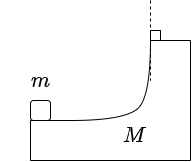
\includegraphics{source/images/energy/energy1.png}

\end{Qbox}

\tcbox[arc is angular, shrink tight, extrude by=4pt]{解答}

物体 \(m\) の右向きの速さが \(M\)
の右向きの速さより大きいと,飛び出すことができないし,逆はあり得ないので,飛び出す際の
\(m,M\) の右の速さは同じであり,それを \(v_x\) とする.
\[v_x=\frac{m}{m+M}v\] ここで,飛び出す瞬間の \(m\) の上向の速さを
\(v_y\) にすると,
\[\frac{1}{2}mv^2=\frac{1}{2}(m+M)v_x^2+\frac{1}{2}mv_y^2+mgh_1\]
\(h_1\) は飛び出す地点の高さである.さらに,飛び出す地点から \(m\)
が到達する最高地点までの鉛直距離 \(h_2\) は \[v_y^2=2gh_2\]
と表せるので,全ての指揮を整理して連立すれば,
\[h_1+h_2=\frac{M}{M+m}\frac{v^2}{2g}\] とわかる.

だがこの問題を一瞬で解決する方法もある.

この問題は, \(t=0\)
の時と,物体が最も高く跳ね上がった瞬間においては,垂直方向の重心速度が0なので,重心運動エネルギーが不変であり,外部への仕事は全て内部運動エネルギーによってなされる.そして,物体
\(m\)
が最も高く飛び上がった瞬間,両物体の相対速さは0となるので,内部運動エネルギーは全て物体
\(m\)
の飛び上がりに使われたとして考えられるので,さらに2体問題であることを考慮して,換算質量を
\(\mu\) とすれば, \[\frac{1}{2}\mu v^2=mgh\]
\[h=\frac{M}{M+m}\frac{v^2}{2g}\] とわかる.

\begin{Qbox}{問題(東京大)}
物体を手のひらにのせ,手をゆっくり上げても物体は手のひらから離れな
いが,手を急激に上げ静止させると物体は手のひらから離れてとび上がる。この
ような現象を模型的に考察してみよう。
図1で示すように,水平面上に平らな台Aがあり,この台の上に質量 \(m\)
の物体Bをのせる。台を水平に保ったまま,図2に示す速度 \(v_A\)
で台を鉛直上方に持ち上げる。台が動きはじめてからの時間を \(T\)
とする。台および物体の鉛直方向の移動距離をそれぞれ \(y_A,y_B\)
とし,重力加速度を \(g\)
とする。物体には空気の抵抗力は働かないものとして,以下の設間に答えよ。a

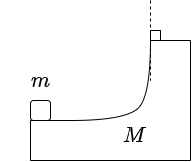
\includegraphics{source/images/energy/energy1.png}

\end{Qbox}

\tcbox[arc is angular, shrink tight, extrude by=4pt]{解答}

\bookmarksetup{startatroot}

\hypertarget{database}{%
\chapter*{DataBase}\label{database}}
\addcontentsline{toc}{chapter}{DataBase}

\markboth{DataBase}{DataBase}

このページではいろいろな大学の過去問,いろいろな参考書の問題番号,IPhOなどの過去問の整理をする.

\begin{longtable}[]{@{}lllll@{}}
\toprule\noalign{}
年度 & 問題 & 分野 & 備考 & 使用 \\
\midrule\noalign{}
\endhead
\bottomrule\noalign{}
\endlastfoot
2019 & 1 & 単振動,力学的エネルギー & & \\
2019 & 2 & 交流,電場,電磁波 & & \\
2019 & 3 & 波動,熱力学 & & \\
2018 & 1 & 万有引力,相対論 & & \\
2018 & 2 & 電場,磁場,量子論 & & \\
2018 & 3 & 流体力学,熱力学 & & \\
2017 & 1 & 万有引力 & & \\
2017 & 2 & 波動,熱力学 & & \\
2017 & 3 & 万有引力,量子論 & & \\
2016 & 1 & 万有引力,角運動量 & & \\
2016 & 2 & 交流 & & \\
\end{longtable}

東大過去問の総評

\begin{longtable}[]{@{}
  >{\raggedright\arraybackslash}p{(\columnwidth - 8\tabcolsep) * \real{0.1000}}
  >{\raggedright\arraybackslash}p{(\columnwidth - 8\tabcolsep) * \real{0.1000}}
  >{\raggedright\arraybackslash}p{(\columnwidth - 8\tabcolsep) * \real{0.1000}}
  >{\raggedright\arraybackslash}p{(\columnwidth - 8\tabcolsep) * \real{0.1333}}
  >{\raggedright\arraybackslash}p{(\columnwidth - 8\tabcolsep) * \real{0.5667}}@{}}
\toprule\noalign{}
\begin{minipage}[b]{\linewidth}\raggedright
年度
\end{minipage} & \begin{minipage}[b]{\linewidth}\raggedright
問題
\end{minipage} & \begin{minipage}[b]{\linewidth}\raggedright
時間
\end{minipage} & \begin{minipage}[b]{\linewidth}\raggedright
難易度
\end{minipage} & \begin{minipage}[b]{\linewidth}\raggedright
感想
\end{minipage} \\
\midrule\noalign{}
\endhead
\bottomrule\noalign{}
\endlastfoot
2023 & 1 & 25分(35) & やや難 &
物理的な話は難しいことはない.誘導に従って解いていけば,問題なく解き切ることはできるだろう.ただし,最後の部分で,数学的に少し面倒な場合分けがあるので,そこは時間がかかるかもしれない \\
2023 & 2 & 15分(16) & 並 &
問題設定が複雑そうに見えるが,そこまで複雑ではない問題.思考を問うような難しい部分は全くなく,誘導で全て時切れる問題.この問題が合否を分けたかもしれない \\
2023 & 3 & 15分(14) & 並 &
熱力学の基本的な問題.ただし入試であまり問われるものではない設定であることと,建前上微積分を使っていないように見せかけて,微積分の知識がないと歯が立たない問題.逆に,しっかりやった人であればボーナスステージになるだろう. \\
\end{longtable}



\end{document}
